\documentclass{beamer}
\usetheme{metropolis}

% specifications for presenter mode
%\beamerdefaultoverlayspecification{<+->}
%\setbeamercovered{transparent}

\usepackage[english]{babel}
\usepackage[utf8x]{inputenc}

%\usepackage{coloremoji}
\usepackage{layout}
\usepackage{multirow}
\usepackage{array}
\usepackage{graphicx}
\graphicspath{ {figs/} }

\setbeameroption{show notes}
\setbeamertemplate{note page}[plain]
\usepackage{listings}
\usepackage{datetime}
\usepackage{url}
\usepackage{tcolorbox}
\usepackage{appendixnumberbeamer}

\usepackage{tikz}
\def\checkmark{\tikz\fill[scale=0.4](0,.35) -- (.25,0) -- (1,.7) -- (.25,.15) -- cycle;}

% math shorthand
\usepackage{bm}
\usepackage{amstext}
\usepackage{amsthm}
\usepackage{amsmath}
\usepackage{mathtools}
\newcommand{\R}{\mathbb{R}}
\newcommand{\D}{\mathcal{D}}
\newcommand{\E}{\mathbb{E}}
\newcommand{\I}{\mathbb{I}}
\newcommand{\pr}{\mathbb{P}}
\newcommand{\F}{\mathcal{F}}
\newcommand{\X}{\mathcal{X}}
\newcommand{\M}{\mathcal{M}}
\newcommand{\lik}{\mathcal{L}}

\newtheorem*{assumption*}{\assumptionnumber}
\providecommand{\assumptionnumber}{}
\makeatletter
\newenvironment{assumption}[2]
 {%
  \renewcommand{\assumptionnumber}{Assumption #1: $\mathcal{#2}$}%
  \begin{assumption*}%
  \protected@edef\@currentlabel{#1: $\mathcal{#2}$}%
 }
 {%
  \end{assumption*}
 }
\makeatother

\DeclarePairedDelimiterX{\infdivx}[2]{(}{)}{%
  #1\;\delimsize\|\;#2%
}
\newcommand{\infdiv}{D\infdivx}
\DeclarePairedDelimiter{\norm}{\lVert}{\rVert}
\DeclareMathOperator*{\argmin}{arg\,min}
\DeclareMathOperator*{\argmax}{arg\,max}

% indepndence notation macro
\newcommand\indep{\protect\mathpalette{\protect\independenT}{\perp}}
\def\independenT#1#2{\mathrel{\rlap{$#1#2$}\mkern2mu{#1#2}}}

% Bibliography
\usepackage{natbib}
\bibpunct{(}{)}{,}{a}{}{;}
\usepackage{bibentry}

% title info
\title{\normalsize Evaluating the causal impacts of vaccine-induced immune
  responses in two-phase vaccine efficacy trials}

\author{\href{https://nimahejazi.org}{Nima Hejazi}\\[-10pt]}

\institute{
  \begin{figure}[!htb]
    \centering
    \begin{minipage}{.65\textwidth}
        Division of Biostatistics, and \\
        Center for Computational Biology, \\
        University of California, Berkeley \\[6pt]
        
\includegraphics[scale=0.12]{twitter-icon.png}
          \href{https://twitter.com/nshejazi}{nshejazi} \\
        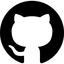
\includegraphics[scale=0.09]{github-icon.png}
          \href{https://github.com/nhejazi}{nhejazi} \\
        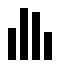
\includegraphics[scale=0.12]{homepage.png}
          \href{https://nimahejazi.org}{nimahejazi.org} \\
      with M.~van der Laan, H.~Janes, P.~Gilbert, D.~Benkeser \\
     Biostatistics seminar, Fred Hutch
    \end{minipage}%
    \begin{minipage}{0.3\textwidth}
      \centering
      
\includegraphics[height=0.70in,width=0.70in]{ucberkeleyseal_874_540.eps}
    \end{minipage}
  \end{figure}
}

\date{Wednesday, 20 January 2021}

%%%%%%%%%%%%%%%%%%%%%%%%%%%%%%%%%%%%%%%%%%%%%%%%%%%%%%%%%%%%%%%%%%%%%%%%%%%%%%%%

% Outline at beginning of each section
%\AtBeginSection[]
%{
  %\begin{frame}<beamer>
    %\frametitle{Outline}
    %\tableofcontents[currentsection]
  %\end{frame}
%}

%%%%%%%%%%%%%%%%%%%%%%%%%%%%%%%%%%%%%%%%%%%%%%%%%%%%%%%%%%%%%%%%%%%%%%%%%%%%%%%%

\begin{document}

\begin{frame}[noframenumbering]
  \thispagestyle{empty}
  \titlepage
\end{frame}

%%%%%%%%%%%%%%%%%%%%%%%%%%%%%%%%%%%%%%%%%%%%%%%%%%%%%%%%%%%%%%%%%%%%%%%%%%%%%%%%

\begin{frame}[c]{The burden of HIV-1}

\begin{center}
\begin{itemize}
  \itemsep10pt
  \item The HIV-1 epidemic --- the facts:
    \begin{itemize}
      \item now in its fourth decade,
      \item 2.5 million new infections occurring annually worldwide,
      \item new infections outpace patients starting antiretroviral therapy.
    \end{itemize}
  \item \textit{Most efficacious} preventive vaccine: $\sim$31\% reduction rate.
  \item \textbf{Question}: To what extent can HIV-1 vaccines be improved by
    modulating immunogenic CD4+/CD8+ response profiles?
\end{itemize}
\end{center}

\note{
}

\end{frame}

%%%%%%%%%%%%%%%%%%%%%%%%%%%%%%%%%%%%%%%%%%%%%%%%%%%%%%%%%%%%%%%%%%%%%%%%%%%%%%%%
\begin{frame}[c]{HVTN 505 trial examined new antibody boost vaccines}

\begin{center}
\begin{itemize}
  \itemsep10pt
  \item HIV Vaccine Trials Network's (HVTN) 505 vaccine efficacy; randomized
    controlled trial, $n = 2504$ \citep{hammer2013efficacy}.
  \item \textbf{Question:} How would HIV-1 infection risk in week 28 have
    changed had vaccine-induced immunogenic response differed?
  \item Immunogenic response profiles only available for second-phase sample of
    $n = 189$ \citep{janes2017higher} due to cost limitations.
  \item \underline{Two-phased sampling mechanism:} 100\% inclusion rate if
    HIV-1 positive in week 28; based on matching otherwise.
\end{itemize}
\end{center}

\note{
\begin{itemize}
  \itemsep10pt
  \item Baseline covariates($L$): sex, age, BMI, behavioral HIV risk.
  \item Intervention(s) ($A$): post-vaccination T-cell activity markers.
  \item Outcome ($Y$): HIV-1 infection status at week 28 of tiral.
  \item 12-color intracellular cytokine staining (ICS) assay.
  \item Cryopreserved peripheral blood mononuclear cells were stimulated with
    synthetic HIV-1 peptide pools.
  \item All immune responses are assayed \textit{after} the endpoints of
    interest (HIV-1 infection status) are collected.
  \item \textbf{Conclusion:} Understanding which immune responses impact vaccine
    efficacy helps develop more efficacious vaccines.
  \item A vaccine effective at preventing HIV-1 acquisition would be a
    cost-effective and durable approach to halting the worldwide epidemic.
  \item Identifying vaccine-induced immune-response biomarkers that predict a
    vaccine's ability to protect individuals from HIV-1 infection is a high
    priority.
  \item The study was halted on 22 April 2013 due to absence of vaccine
    efficacy. There was no significant effect of the vaccine on the primary
    infection endpoint of HIV-1 infection between week 28 and month 24.
\end{itemize}
}

\end{frame}

%%%%%%%%%%%%%%%%%%%%%%%%%%%%%%%%%%%%%%%%%%%%%%%%%%%%%%%%%%%%%%%%%%%%%%%%%%%%%%%%

\begin{frame}[c]{Two-phase sampling censors the complete data structure}

\begin{center}
\begin{itemize}
  \itemsep10pt
  \item Complete (\underline{unobserved}) data $X = (L, A, S, Y) \sim P_0^X \in
    \mathcal{M}^X$, as per the full HVTN 505 trial cohort
    \citep{hammer2013efficacy}:
    \vspace{1em}
    \begin{itemize}
      \itemsep8pt
      \item $L$ (baseline covariates): sex, age, BMI, behavioral HIV risk,
      \item $A$ (treatment): vaccination status (randomized),
      \item $S$ (exposure): immune response profile for CD4+ and CD8+,
      \item $Y$ (outcome of interest): HIV-1 infection status at week 28.
    \end{itemize}
  \item Observed data $O = (C, C X) = (L, C, C S, Y)$.
    \vspace{1em}
    \begin{itemize}
      \itemsep8pt
      \item $C \in \{0,1\}$ indicates inclusion in the second-phase sample.
      \item Implicitly conditioning on the vaccine arm, i.e., $O = X \mid A = 1$.
    \end{itemize}
\end{itemize}
\end{center}

\note{
  \begin{itemize}
    \item $P_0^X$ --- true (unknown) distribution of the full data $X$,
    \item $\mathcal{M}^X_{NP}$ --- nonparametric statistical model.
  \end{itemize}
}

\end{frame}

%%%%%%%%%%%%%%%%%%%%%%%%%%%%%%%%%%%%%%%%%%%%%%%%%%%%%%%%%%%%%%%%%%%%%%%%%%%%%%%%

\begin{frame}[c]{NPSEM with static interventions}

\begin{center}
\begin{itemize}
  \itemsep10pt
  \item Use a nonparametric structural equation model (NPSEM) to describe the
    generation of $X$ \citep{pearl2009causality}, specifically
    \begin{equation*}
      L = f_L(U_L); S = f_S(L, U_S); Y = f_Y(S, L, U_Y)
    \end{equation*}
  \item Implies a model for the distribution of counterfactual random variables
    generated by interventions on the process.
  \item A \textit{static intervention} replaces $f_S$ with a specific value $s$
    in its conditional support $S \mid A = 1, L$.
  \item This requires specifying a particular value of the exposure under which
    to evaluate the outcome \textit{a priori}.
\end{itemize}
\end{center}

\note{
}

\end{frame}

%%%%%%%%%%%%%%%%%%%%%%%%%%%%%%%%%%%%%%%%%%%%%%%%%%%%%%%%%%%%%%%%%%%%%%%%%%%%%%%%

\begin{frame}[c]{NPSEM with stochastic interventions}

\begin{center}
\begin{itemize}
  \itemsep10pt
  \item \textit{Stochastic interventions} modify the value $S$ would naturally
    assume by drawing from a modified exposure distribution.
  \item Consider the post-intervention value $S^{\star} \sim G^{\star}(\cdot
    \mid L)$; static interventions are a special case (degenerate distribution).
  \item Such an intervention generates a counterfactual random variable
    $Y_{G^{\star}} \coloneqq f_Y(S^{\star}, L, U_Y)$, with distribution
    $P_0^{\delta}$, .
  \item We aim to estimate $\psi_{0,\delta} \coloneqq \E_{P_0^{\delta}}
    \{Y_{G^{\star}}\}$, the counterfactual mean under the post-intervention
    exposure distribution $G^{\star}$.
\end{itemize}
\end{center}

\note{
}

\end{frame}

%%%%%%%%%%%%%%%%%%%%%%%%%%%%%%%%%%%%%%%%%%%%%%%%%%%%%%%%%%%%%%%%%%%%%%%%%%%%%%%%

\begin{frame}[c]{Stochastic interventions for the causal effects of shifts}

\begin{center}
\begin{itemize}
  \itemsep10pt
  \item \cite{diaz2012population, diaz2018stochastic}'s \textit{stochastic}
    interventions
     \begin{equation*}\label{shift_intervention}
       d(s, l) =
         \begin{cases}
           s + \delta, & s + \delta < u(l) \quad (\text{if plausible}) \\
           s, & s + \delta \geq u(l) \quad (\text{otherwise})
         \end{cases}
     \end{equation*}
  \item Our estimand is $\psi_{0, d} \coloneqq \E_{P_0^d}\{Y_{d(S,L)}\}$, mean
    of $Y_{d(S, L)}$.
  \item Statistical target parameter is
    $\Psi(P_0^X) = \E_{P_0^X}{\overline{Q}(d(S, L), L)}$, counterfactual mean
    of the \textit{shifted} outcome mechanism.
  \item For HVTN 505, $\psi_{0,d}$ is the counterfactual risk of HIV-1
    infection, had the observed value of the immune response been altered under
    the rule $d(S,L)$ defining $G^{\star}(\cdot \mid L)$.
\end{itemize}
\end{center}

\note{
  \begin{itemize}
  \item Causal estimand: counterfactual mean of HIV-1 infection (risk) under a
    \textit{shifted} immunogenic response distribution.
  \end{itemize}
}

\end{frame}

%%%%%%%%%%%%%%%%%%%%%%%%%%%%%%%%%%%%%%%%%%%%%%%%%%%%%%%%%%%%%%%%%%%%%%%%%%%%%%%%

\begin{frame}[c]{From the causal to the statistical target parameter}

\begin{center}
\begin{tcolorbox}
\begin{assumption}{1}{\textit{Stable Unit Treatment Value (SUTVA)}}\label{sutva}
  \begin{itemize}
      \itemsep4pt
    \item $Y^{d(s_i, l_i)}_i$ does not depend on $d(s_j, l_j)$ for
        $i = 1, \ldots, n$ and $j \neq i$, or lack of interference
        \citep{rubin1978bayesian, rubin1980randomization}
     \item $Y^{d(s_i, l_i)}_i = Y_i$ in the event $S_i = d(s_i, l_i)$, for
        $i = 1, \ldots, n$
  \end{itemize}
\end{assumption}
\end{tcolorbox}
\vspace{-0.5em}
\begin{tcolorbox}
\begin{assumption}{2}{\textit{Ignorability}}\label{ignorability}
  $S_i \indep Y^{d(s_i, l_i)}_i \mid L_i$, for $i = 1, \ldots, n$
\end{assumption}
\end{tcolorbox}
\vspace{-0.5em}
\begin{tcolorbox}
\begin{assumption}{3}{\textit{Positivity}}\label{positivity}
  $s_i \in \mathcal{S} \implies d(s_i, l_i) \in \mathcal{S}$ for all
  $l \in \mathcal{L}$, where $\mathcal{S}$ denotes the support of $S$
  conditional on $L = l_i$ for all $i = 1, \ldots n$
\end{assumption}
\end{tcolorbox}
\end{center}

\note{
\begin{itemize}
  \itemsep4pt
  \item This positivity assumption is not quite the same as that required for
    categorical interventions.
  \item In particular, we do not require that the intervention density place
    mass across all strata defined by $L$.
  \item Rather, we merely require the post-intervention quantity be seen in the
    observed data for given $s_i \in \mathcal{S}$ and $l_i \in \mathcal{L}$.
\end{itemize}
}

\end{frame}

%%%%%%%%%%%%%%%%%%%%%%%%%%%%%%%%%%%%%%%%%%%%%%%%%%%%%%%%%%%%%%%%%%%%%%%%%%%%%%%%

\begin{frame}[c]{Literature: \cite{diaz2012population}}

\begin{center}
\begin{itemize}
  \itemsep10pt
  \item \textit{Proposal:} Evaluate outcome under an altered
    \textit{intervention distribution} --- e.g.,
    $P_{\delta}(g_0)(S = s \mid L) = g_0(s - \delta(L) \mid L)$.
  \item Identification conditions for a statistical parameter of the
    counterfactual outcome $\psi_{0,d}$ under such an intervention.
  \item Show that the causal quantity of interest $\E_0 \{Y_{d(S, L)}\}$ is
    identified by a functional of the distribution of $X$:
    \begin{align*}\label{eqn:identification2012}
      \psi_{0,d} = \int_{\mathcal{L}} \int_{\mathcal{S}} &\E_{P_0^X} \{Y \mid
        S = d(s, l), L = l\} \cdot \\ &q_{0, S}^X(s \mid L = l) \cdot
        q_{0, L}^X(l) d\mu(s)d\nu(l)
    \end{align*}
  \item Provides a derivation based on the efficient influence function (EIF)
    with respect to the nonparametric model $\mathcal{M}$.
\end{itemize}
\end{center}

\note{
  \begin{itemize}
    \item The identification result allows us to write down the causal quantity
      of interest in terms of a functional of the observed data.
    \item Key innovation: loosening standard assumptions through a change in
      the observed intervention mechanism.
    \item Problem: globally altering an intervention mechanism does not
      necessarily respect individual characteristics.
    \item The authors build IPW, one-step, and TML estimators, comparing the
      three different approaches.
  \end{itemize}
}

\end{frame}

%%%%%%%%%%%%%%%%%%%%%%%%%%%%%%%%%%%%%%%%%%%%%%%%%%%%%%%%%%%%%%%%%%%%%%%%%%%%%%%%

\begin{frame}[c]{HIV-1 risk under shifted immunogenic responses}

%\centering
\hspace*{-1cm}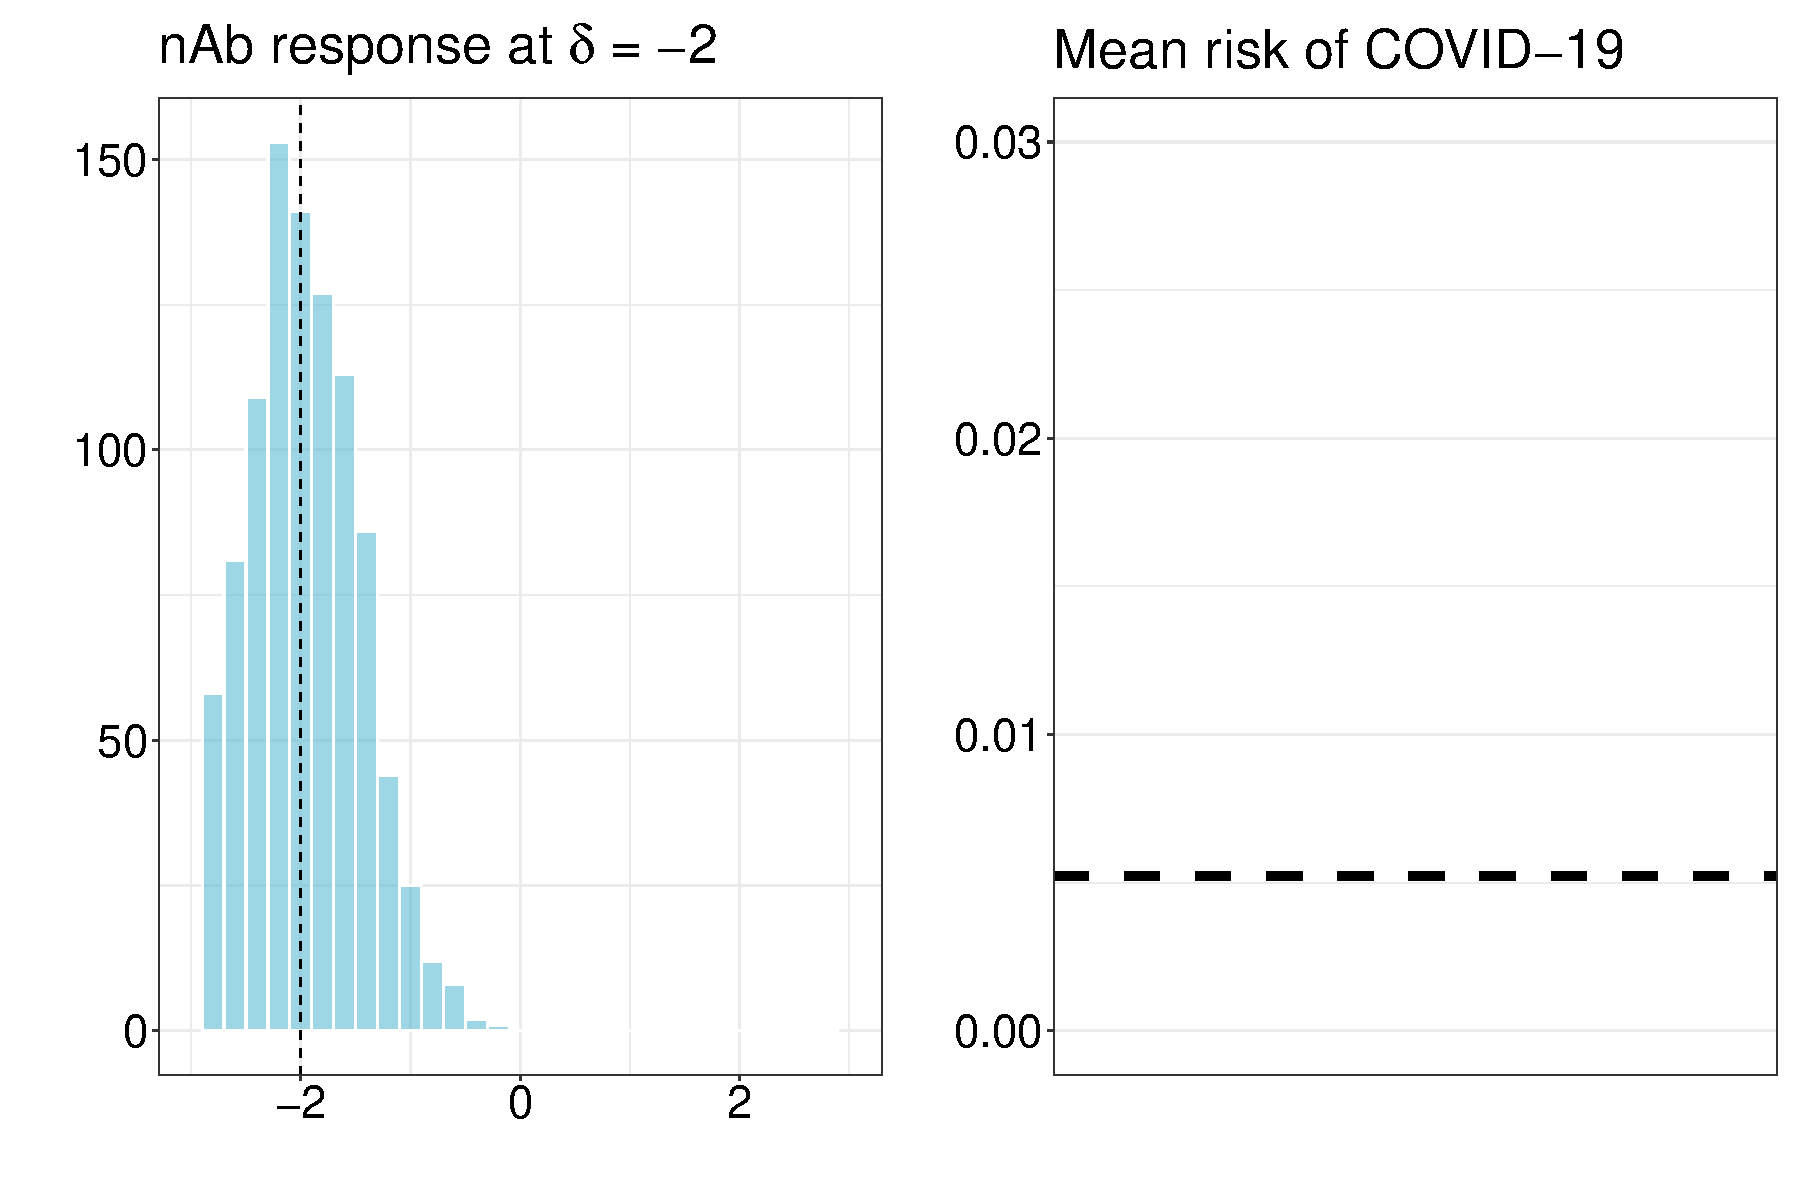
\includegraphics[scale=0.4]{shift-1}

\note{
}

\end{frame}

%%%%%%%%%%%%%%%%%%%%%%%%%%%%%%%%%%%%%%%%%%%%%%%%%%%%%%%%%%%%%%%%%%%%%%%%%%%%%%%%

\begin{frame}[c,noframenumbering]{HIV-1 risk under shifted immunogenic responses}

%\centering
\hspace*{-1cm}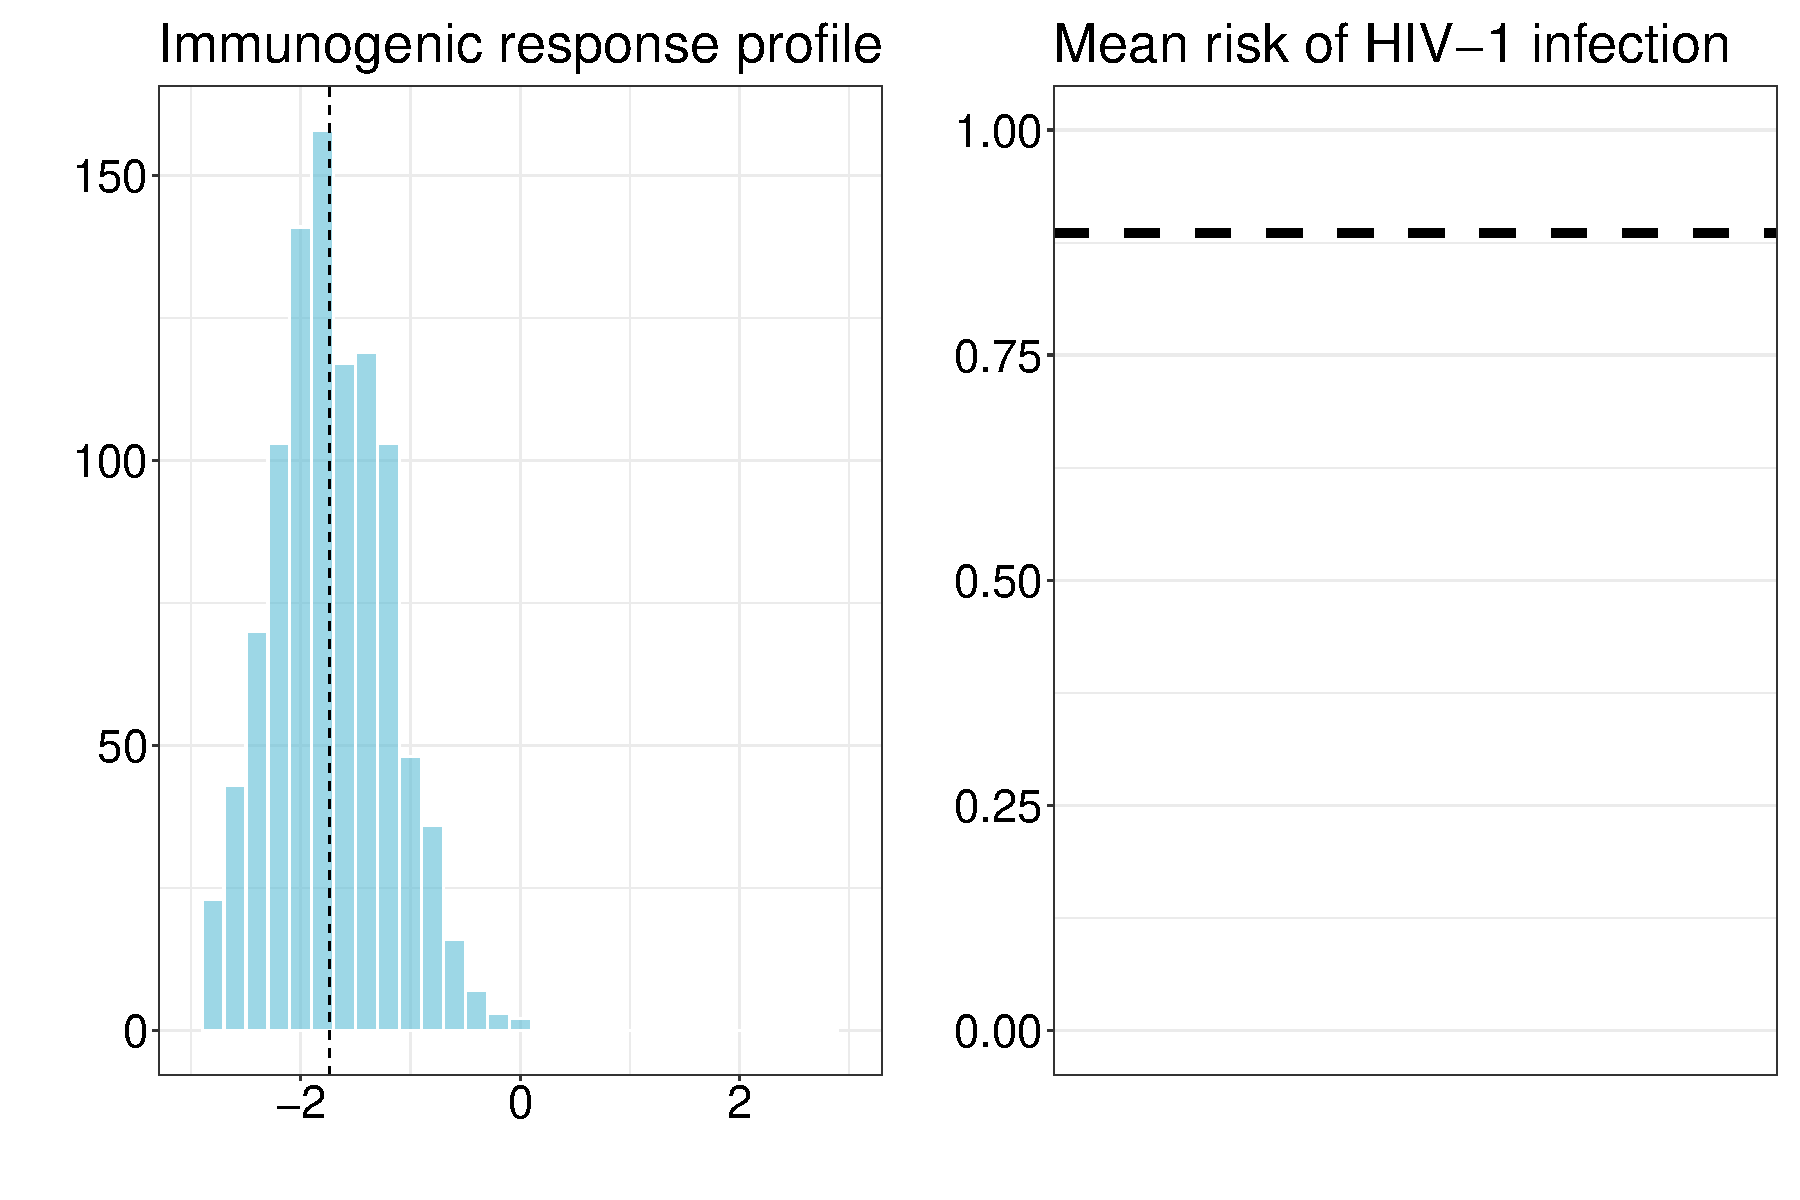
\includegraphics[scale=0.4]{shift-2}

\note{
}

\end{frame}

%%%%%%%%%%%%%%%%%%%%%%%%%%%%%%%%%%%%%%%%%%%%%%%%%%%%%%%%%%%%%%%%%%%%%%%%%%%%%%%%

\begin{frame}[c,noframenumbering]{HIV-1 risk under shifted immunogenic responses}

%\centering
\hspace*{-1cm}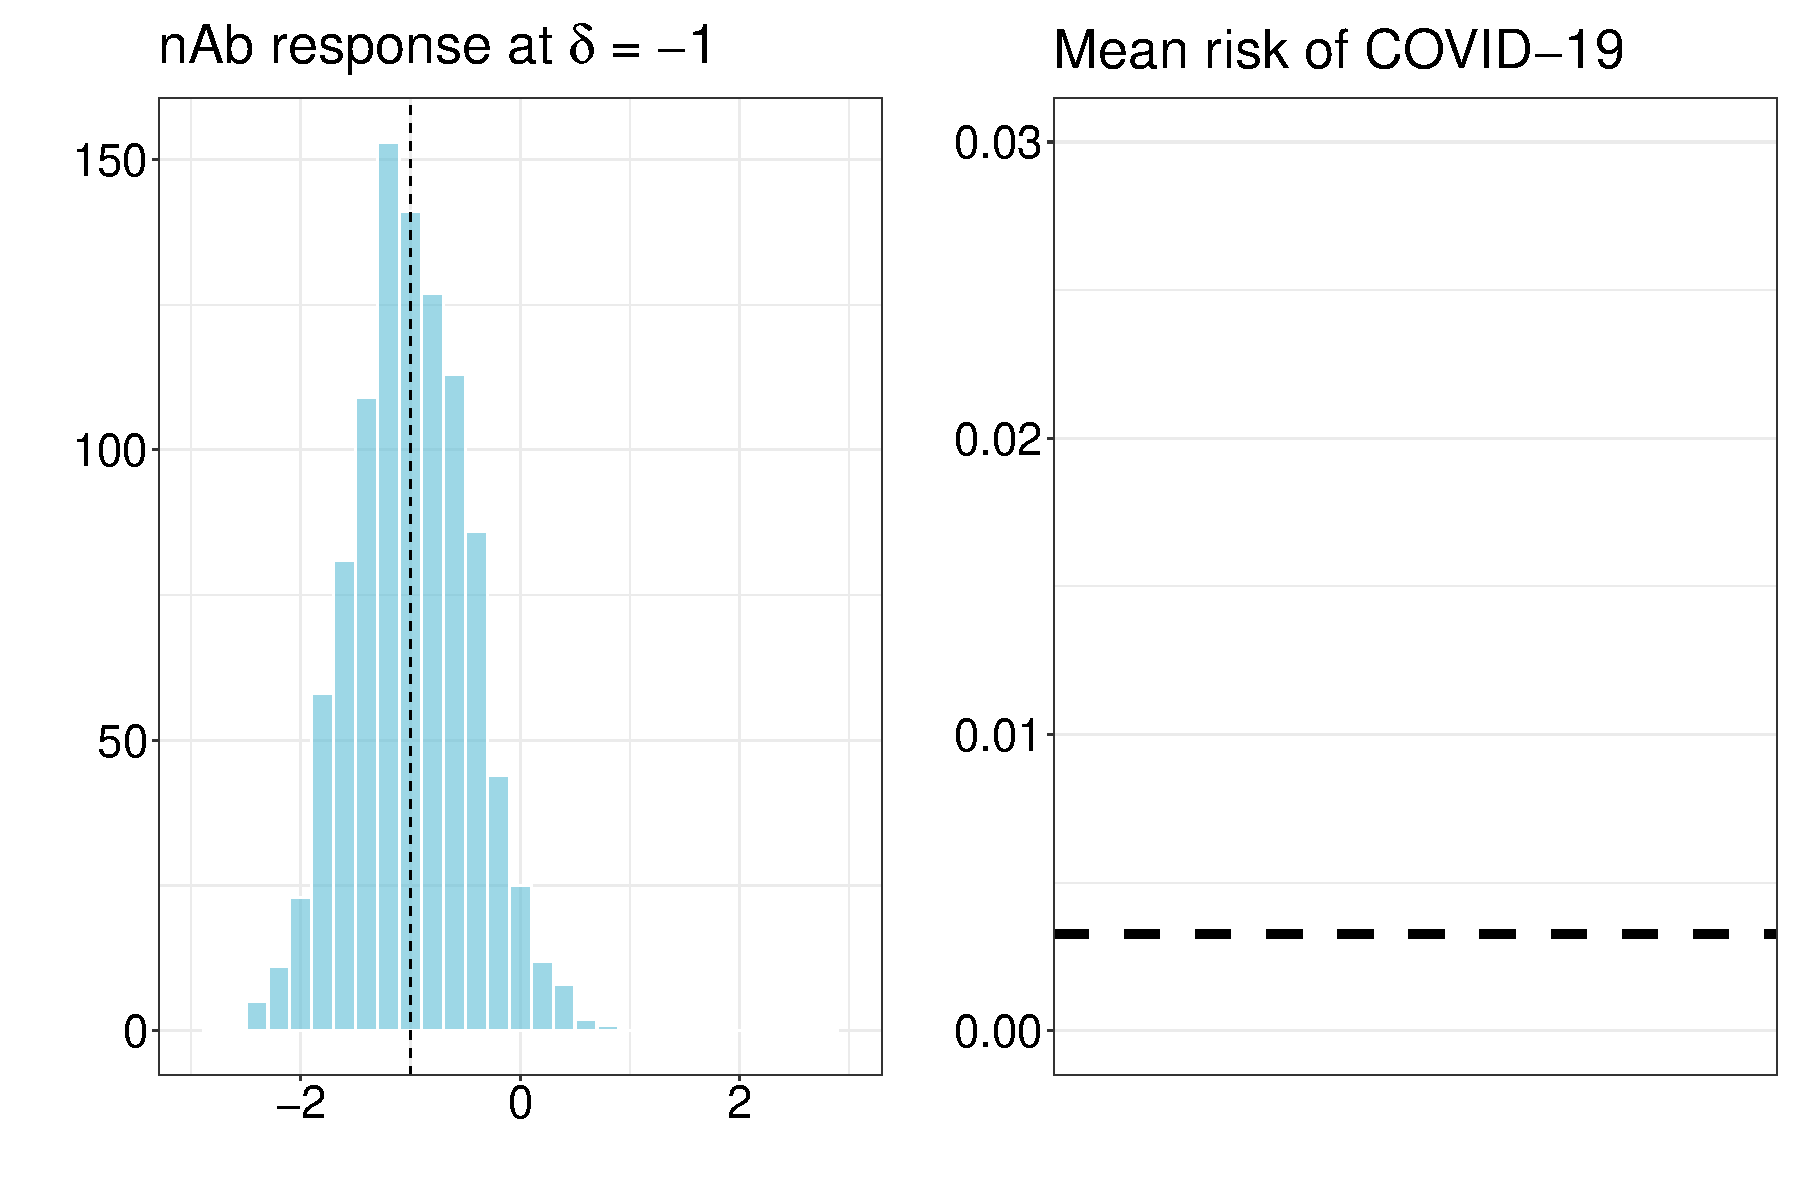
\includegraphics[scale=0.4]{shift-3}

\note{
}

\end{frame}

%%%%%%%%%%%%%%%%%%%%%%%%%%%%%%%%%%%%%%%%%%%%%%%%%%%%%%%%%%%%%%%%%%%%%%%%%%%%%%%%

\begin{frame}[c,noframenumbering]{HIV-1 risk under shifted immunogenic responses}

%\centering
\hspace*{-1cm}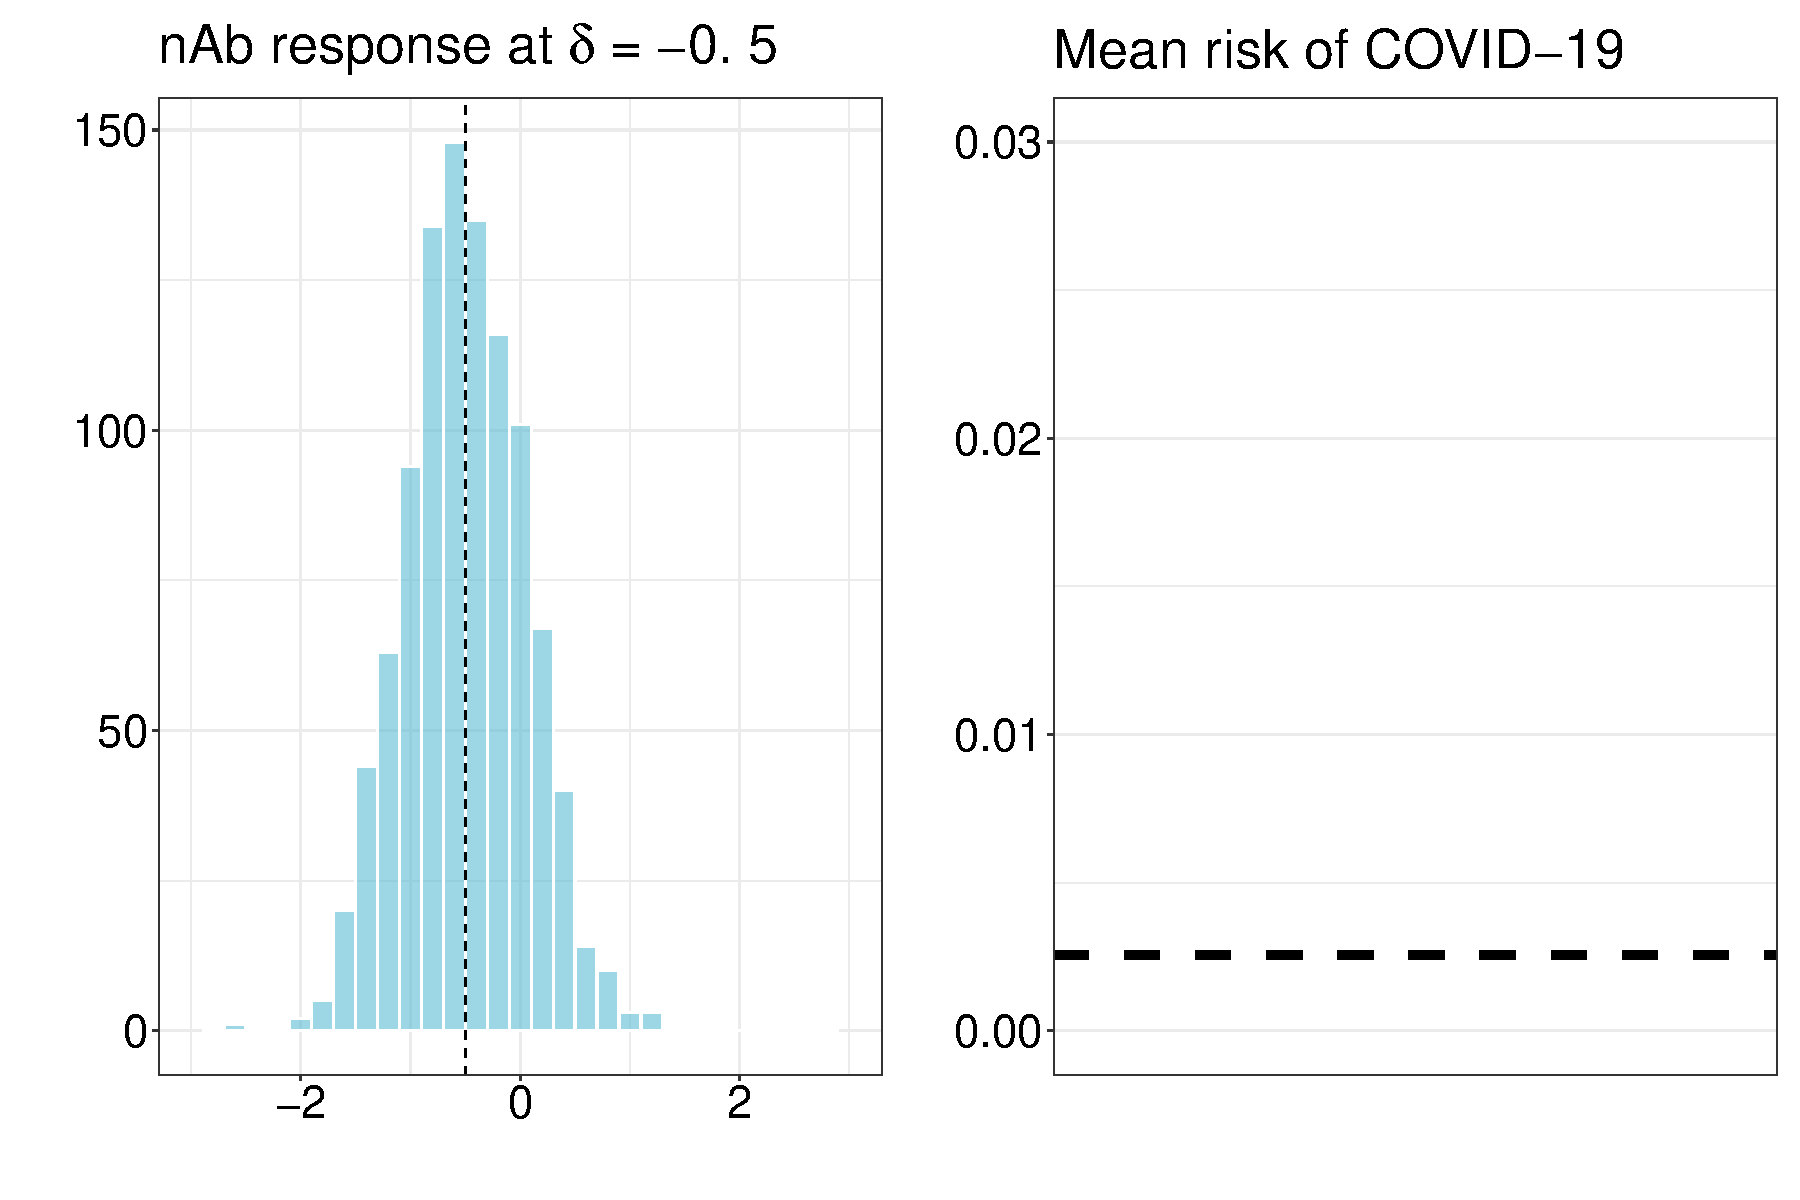
\includegraphics[scale=0.4]{shift-4}

\note{
}

\end{frame}

%%%%%%%%%%%%%%%%%%%%%%%%%%%%%%%%%%%%%%%%%%%%%%%%%%%%%%%%%%%%%%%%%%%%%%%%%%%%%%%%

\begin{frame}[c,noframenumbering]{HIV-1 risk under shifted immunogenic responses}

%\centering
\hspace*{-1cm}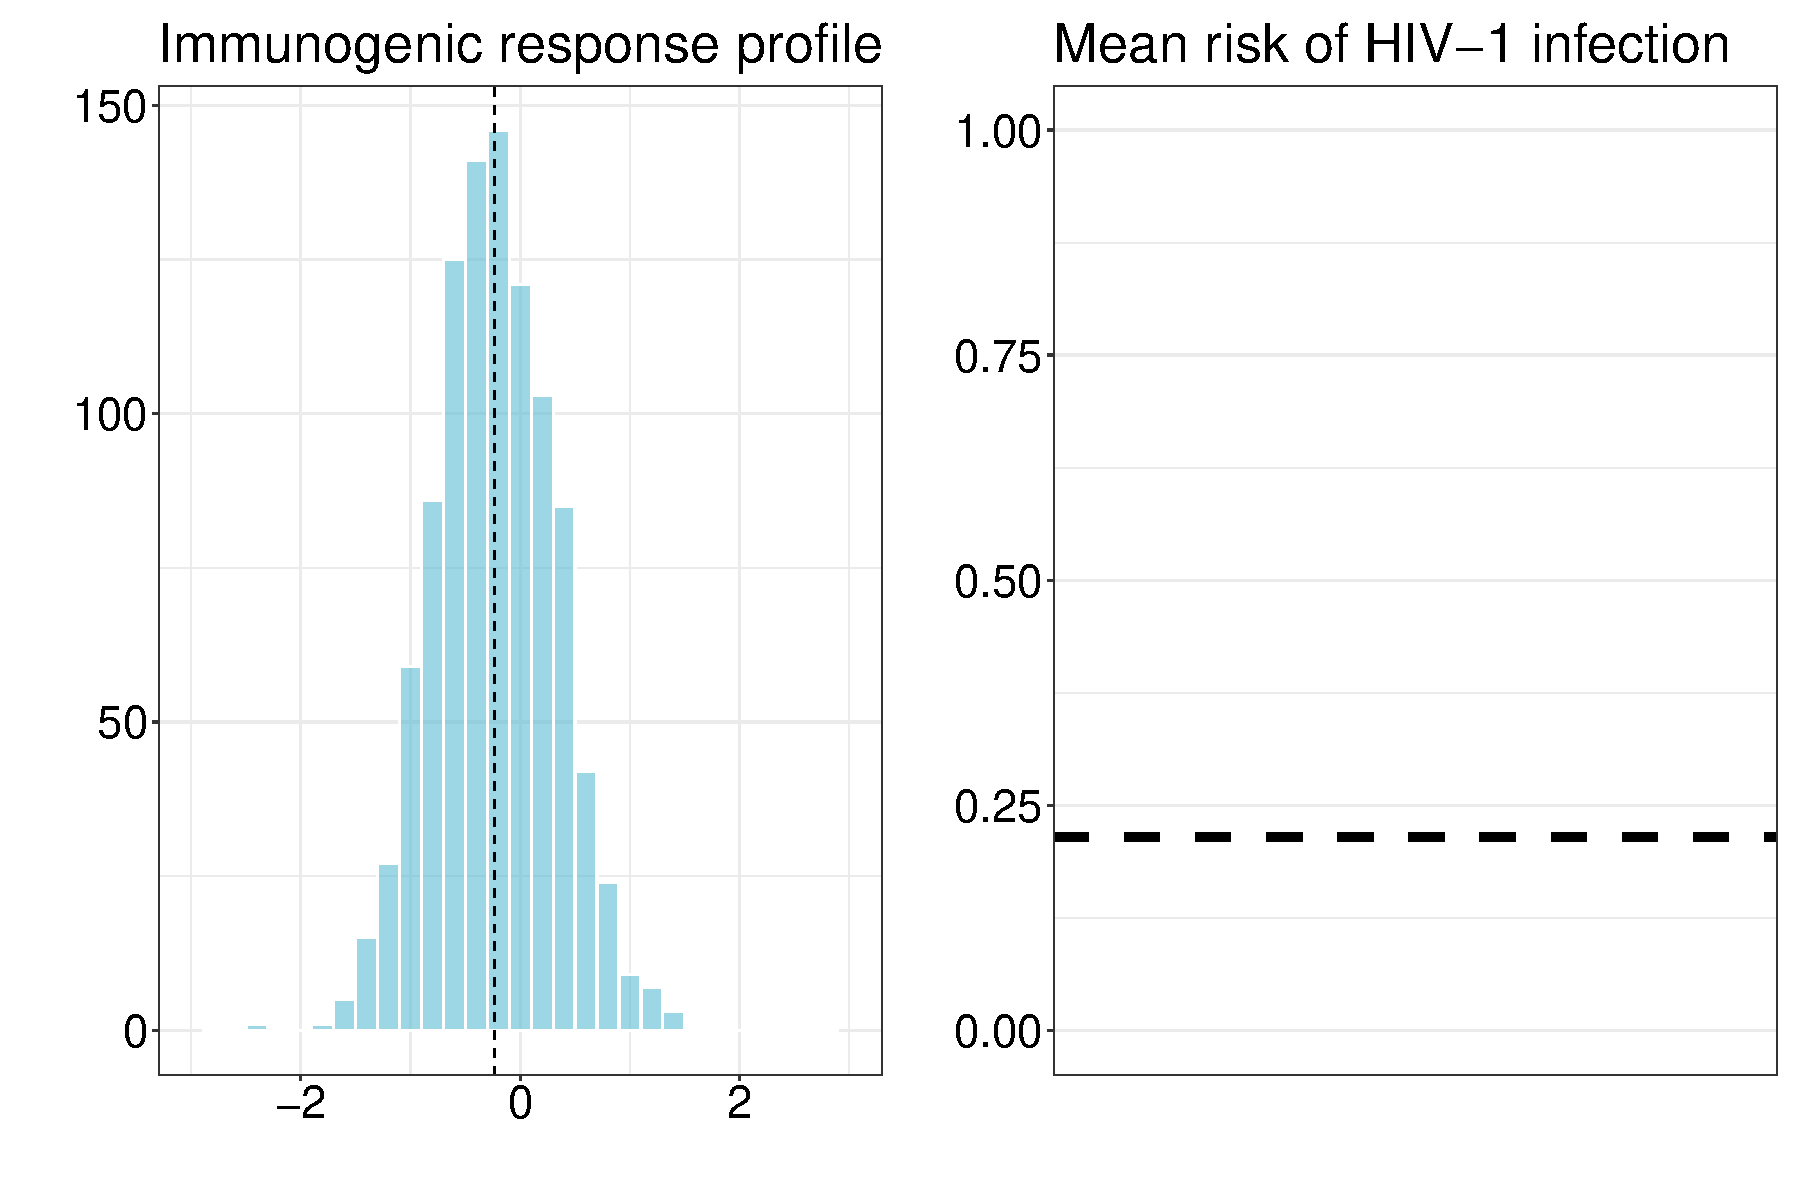
\includegraphics[scale=0.4]{shift-5}

\note{
}

\end{frame}

%%%%%%%%%%%%%%%%%%%%%%%%%%%%%%%%%%%%%%%%%%%%%%%%%%%%%%%%%%%%%%%%%%%%%%%%%%%%%%%%

\begin{frame}[c,noframenumbering]{HIV-1 risk under shifted immunogenic responses}

%\centering
\hspace*{-1cm}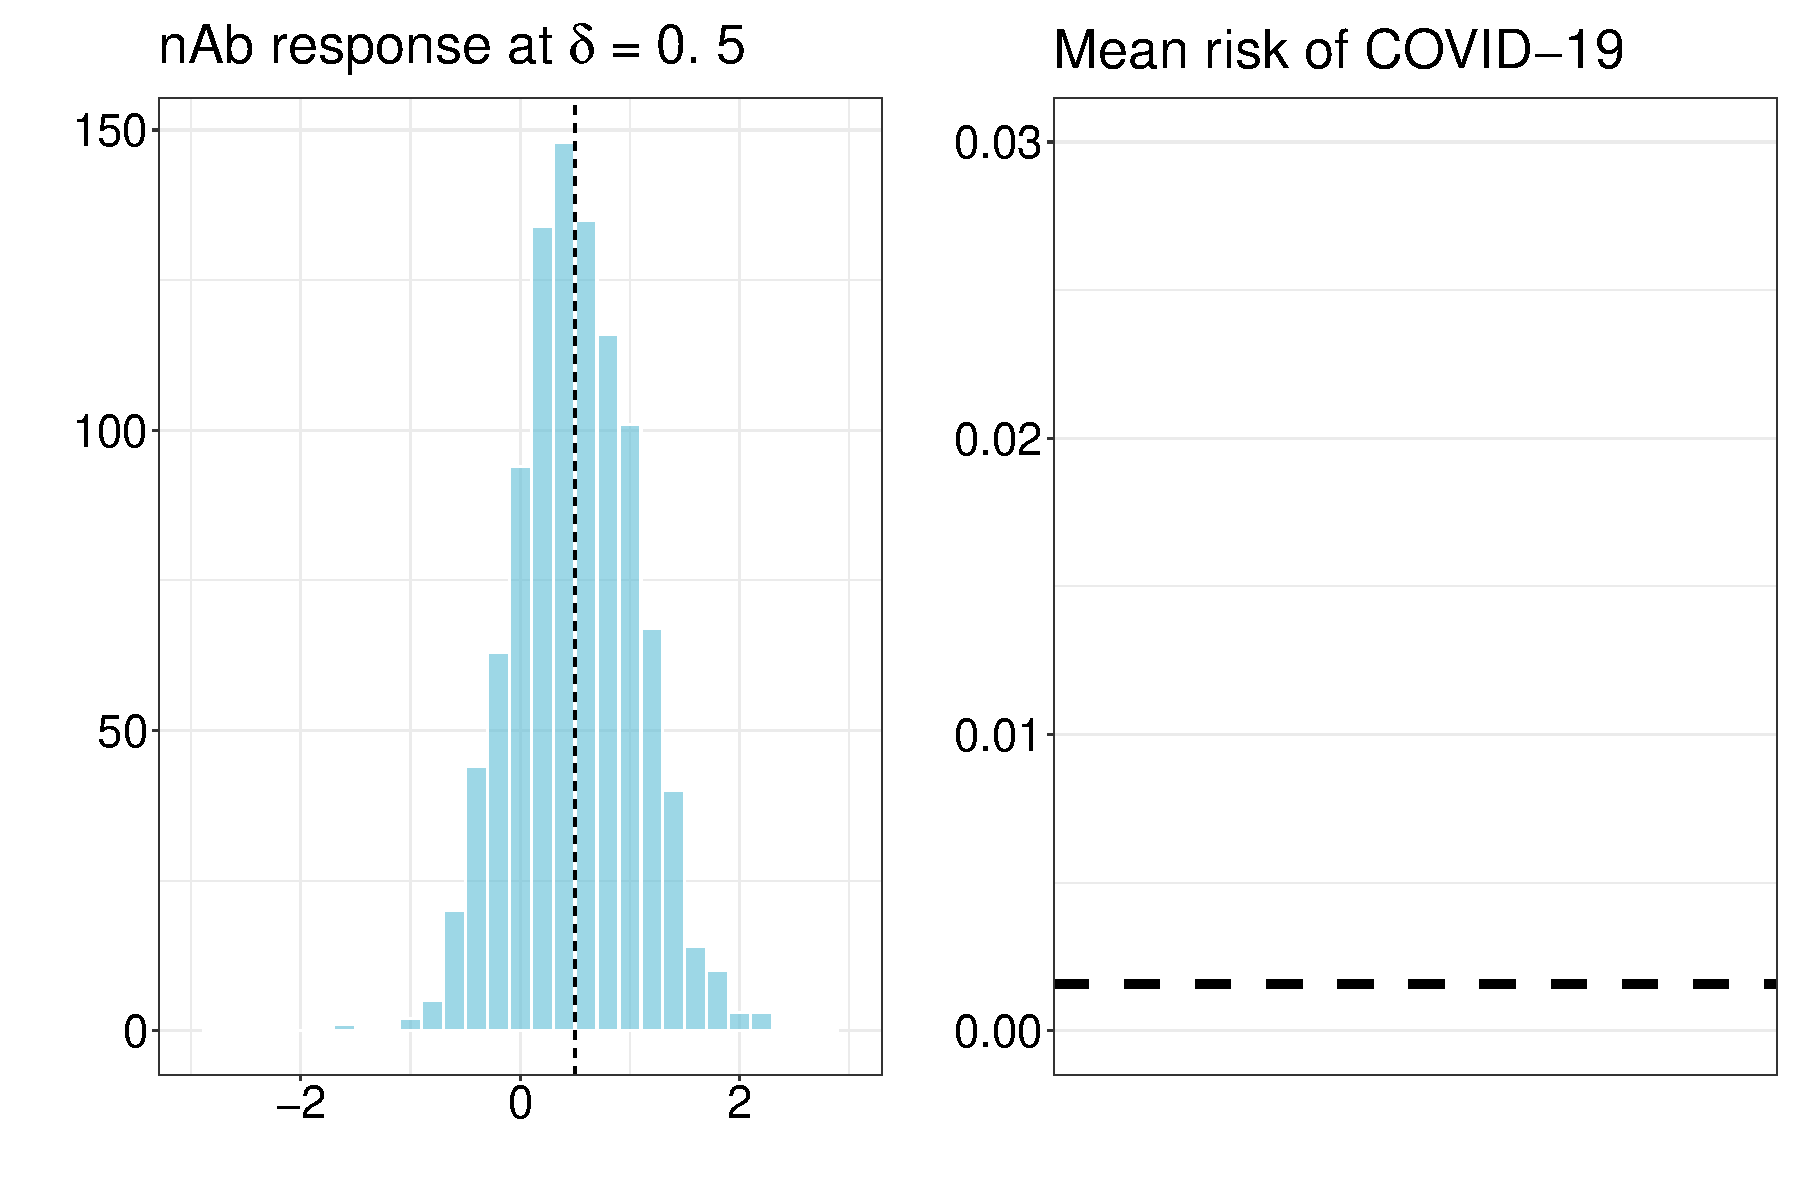
\includegraphics[scale=0.4]{shift-6}

\note{
}

\end{frame}

%%%%%%%%%%%%%%%%%%%%%%%%%%%%%%%%%%%%%%%%%%%%%%%%%%%%%%%%%%%%%%%%%%%%%%%%%%%%%%%%

\begin{frame}[c,noframenumbering]{HIV-1 risk under shifted immunogenic responses}

%\centering
\hspace*{-1cm}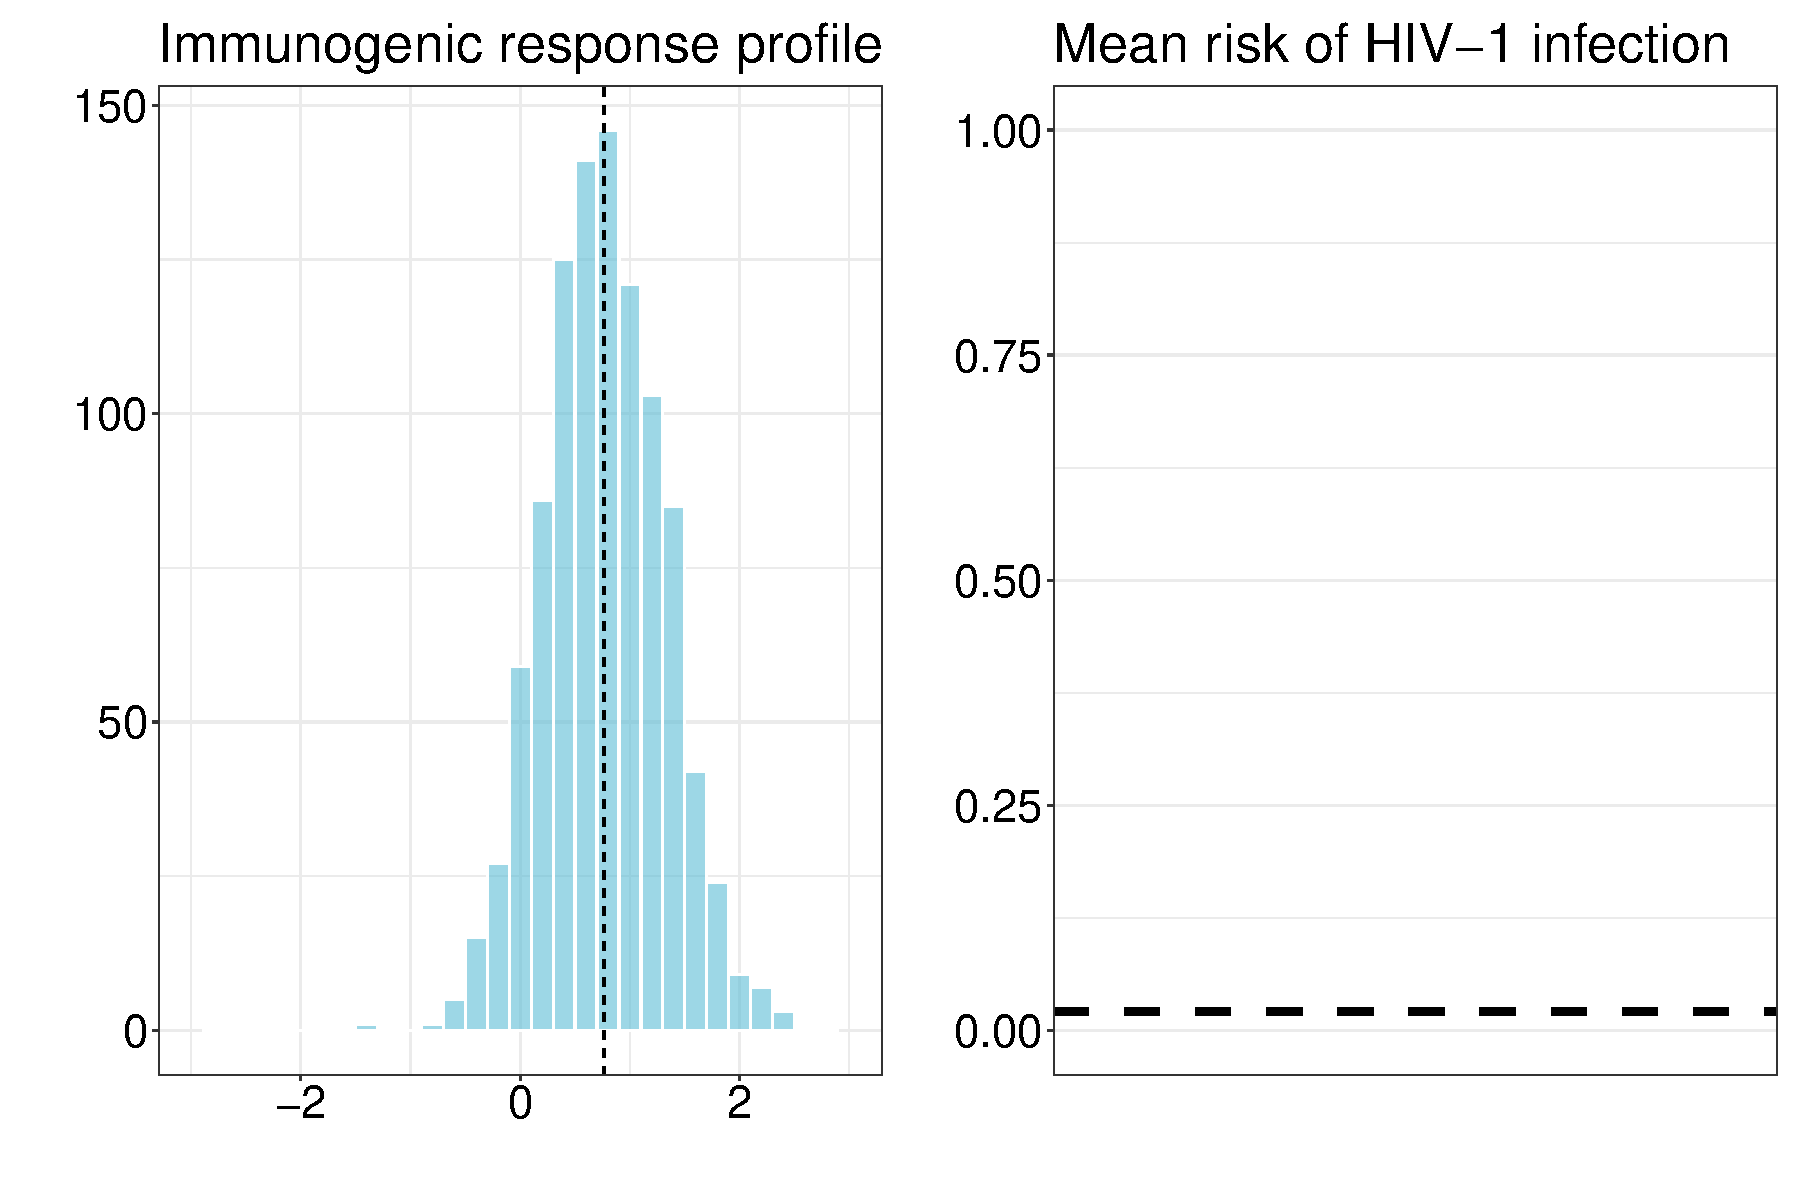
\includegraphics[scale=0.4]{shift-7}

\note{
}

\end{frame}

%%%%%%%%%%%%%%%%%%%%%%%%%%%%%%%%%%%%%%%%%%%%%%%%%%%%%%%%%%%%%%%%%%%%%%%%%%%%%%%%

\begin{frame}[c,noframenumbering]{HIV-1 risk under shifted immunogenic responses}

%\centering
\hspace*{-1cm}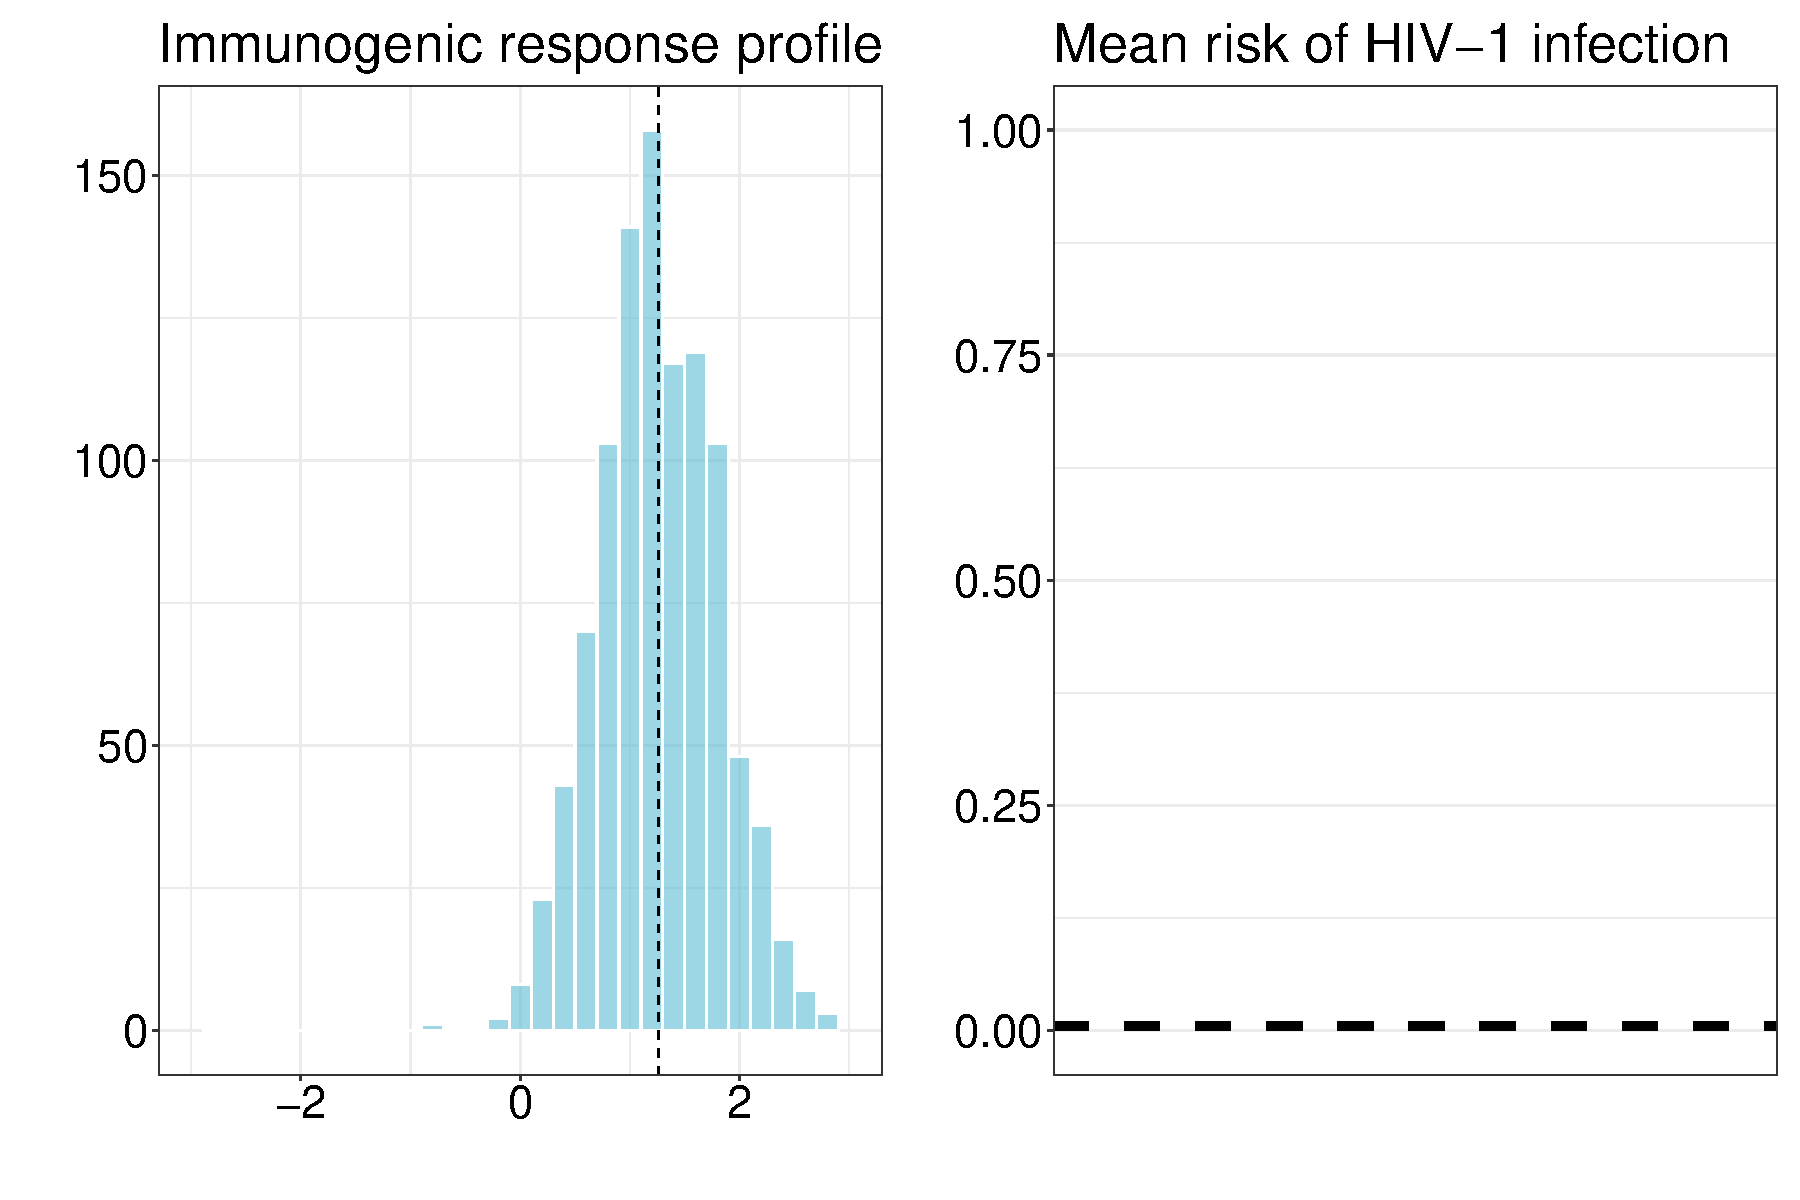
\includegraphics[scale=0.4]{shift-8}

\note{
}

\end{frame}

%%%%%%%%%%%%%%%%%%%%%%%%%%%%%%%%%%%%%%%%%%%%%%%%%%%%%%%%%%%%%%%%%%%%%%%%%%%%%%%%

\begin{frame}[c,noframenumbering]{HIV-1 risk under shifted immunogenic responses}

%\centering
\hspace*{-1cm}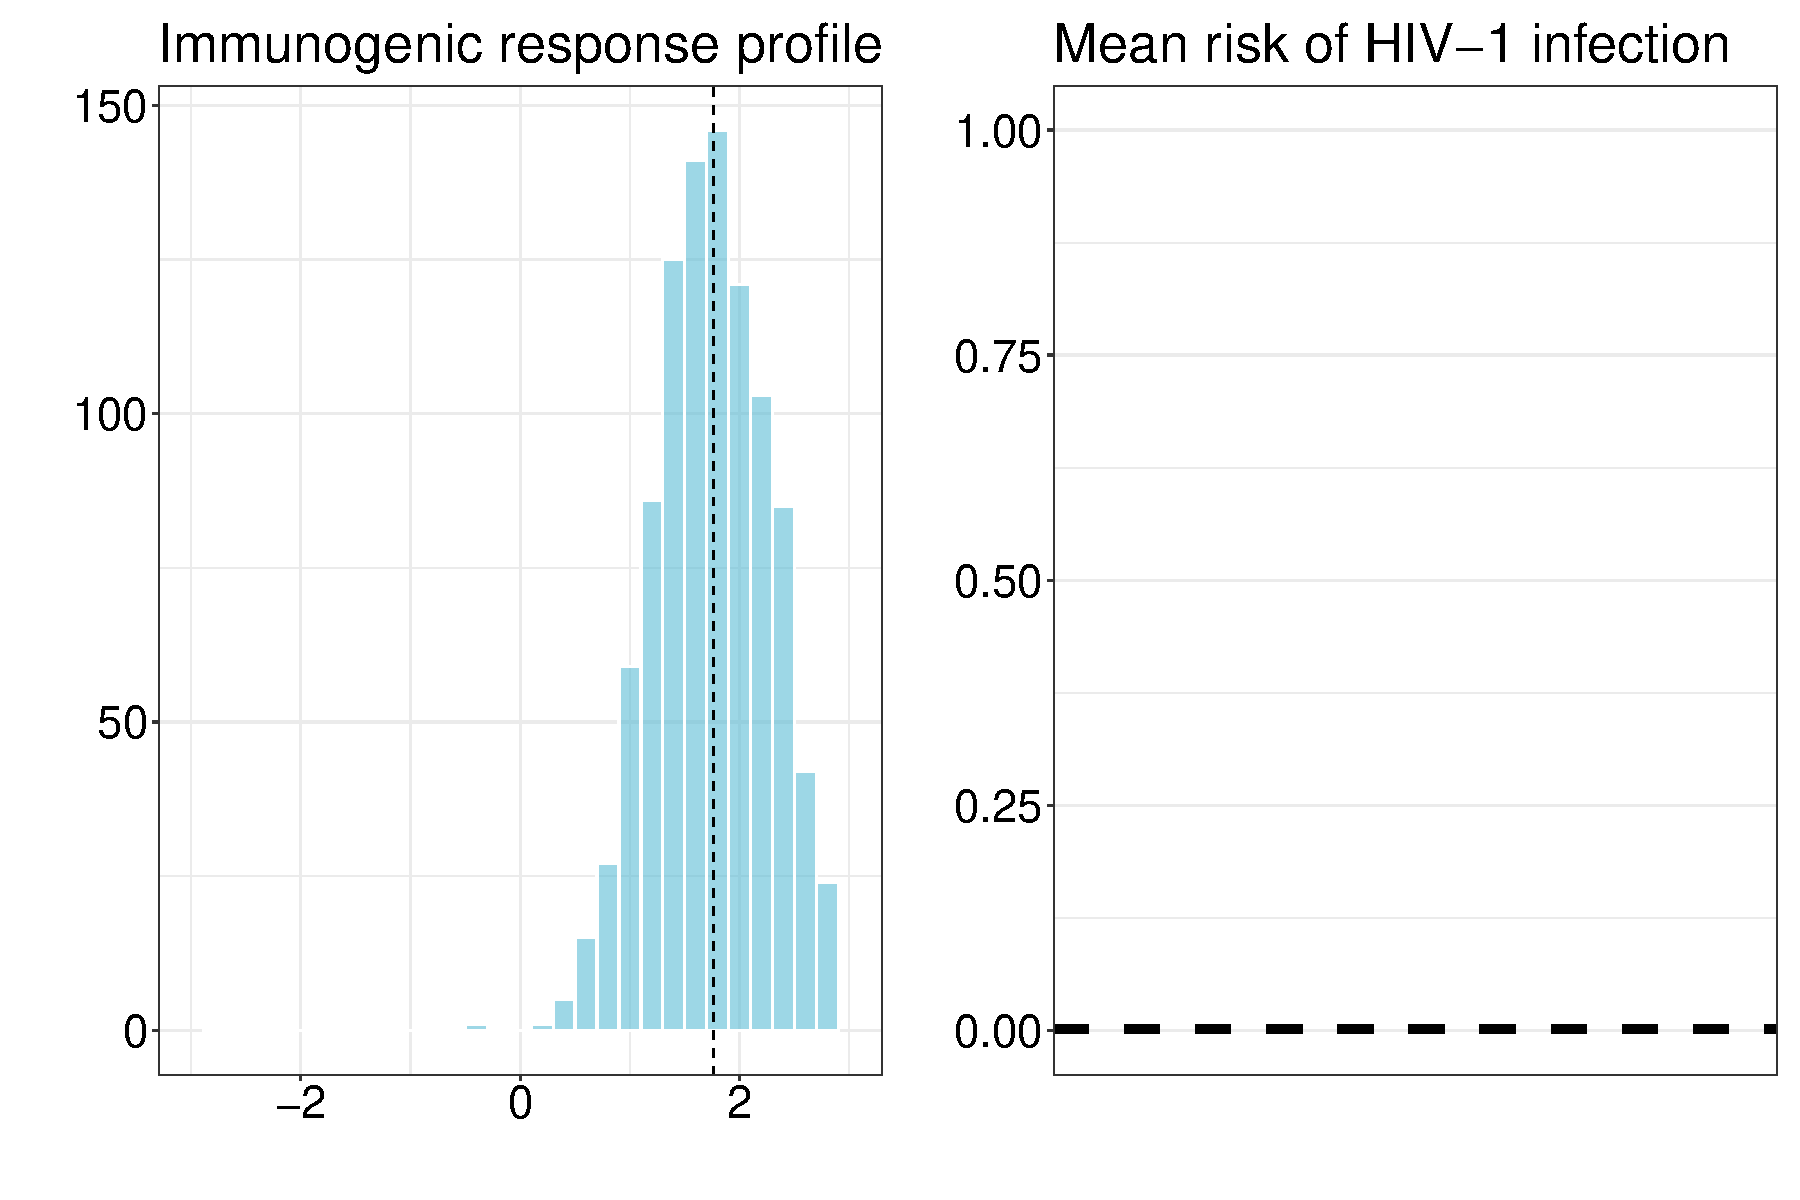
\includegraphics[scale=0.4]{shift-9}

\note{
}

\end{frame}

%%%%%%%%%%%%%%%%%%%%%%%%%%%%%%%%%%%%%%%%%%%%%%%%%%%%%%%%%%%%%%%%%%%%%%%%%%%%%%%%

\begin{frame}[c,noframenumbering]{HIV-1 risk under shifted immunogenic responses}

%\centering
\hspace*{-1cm}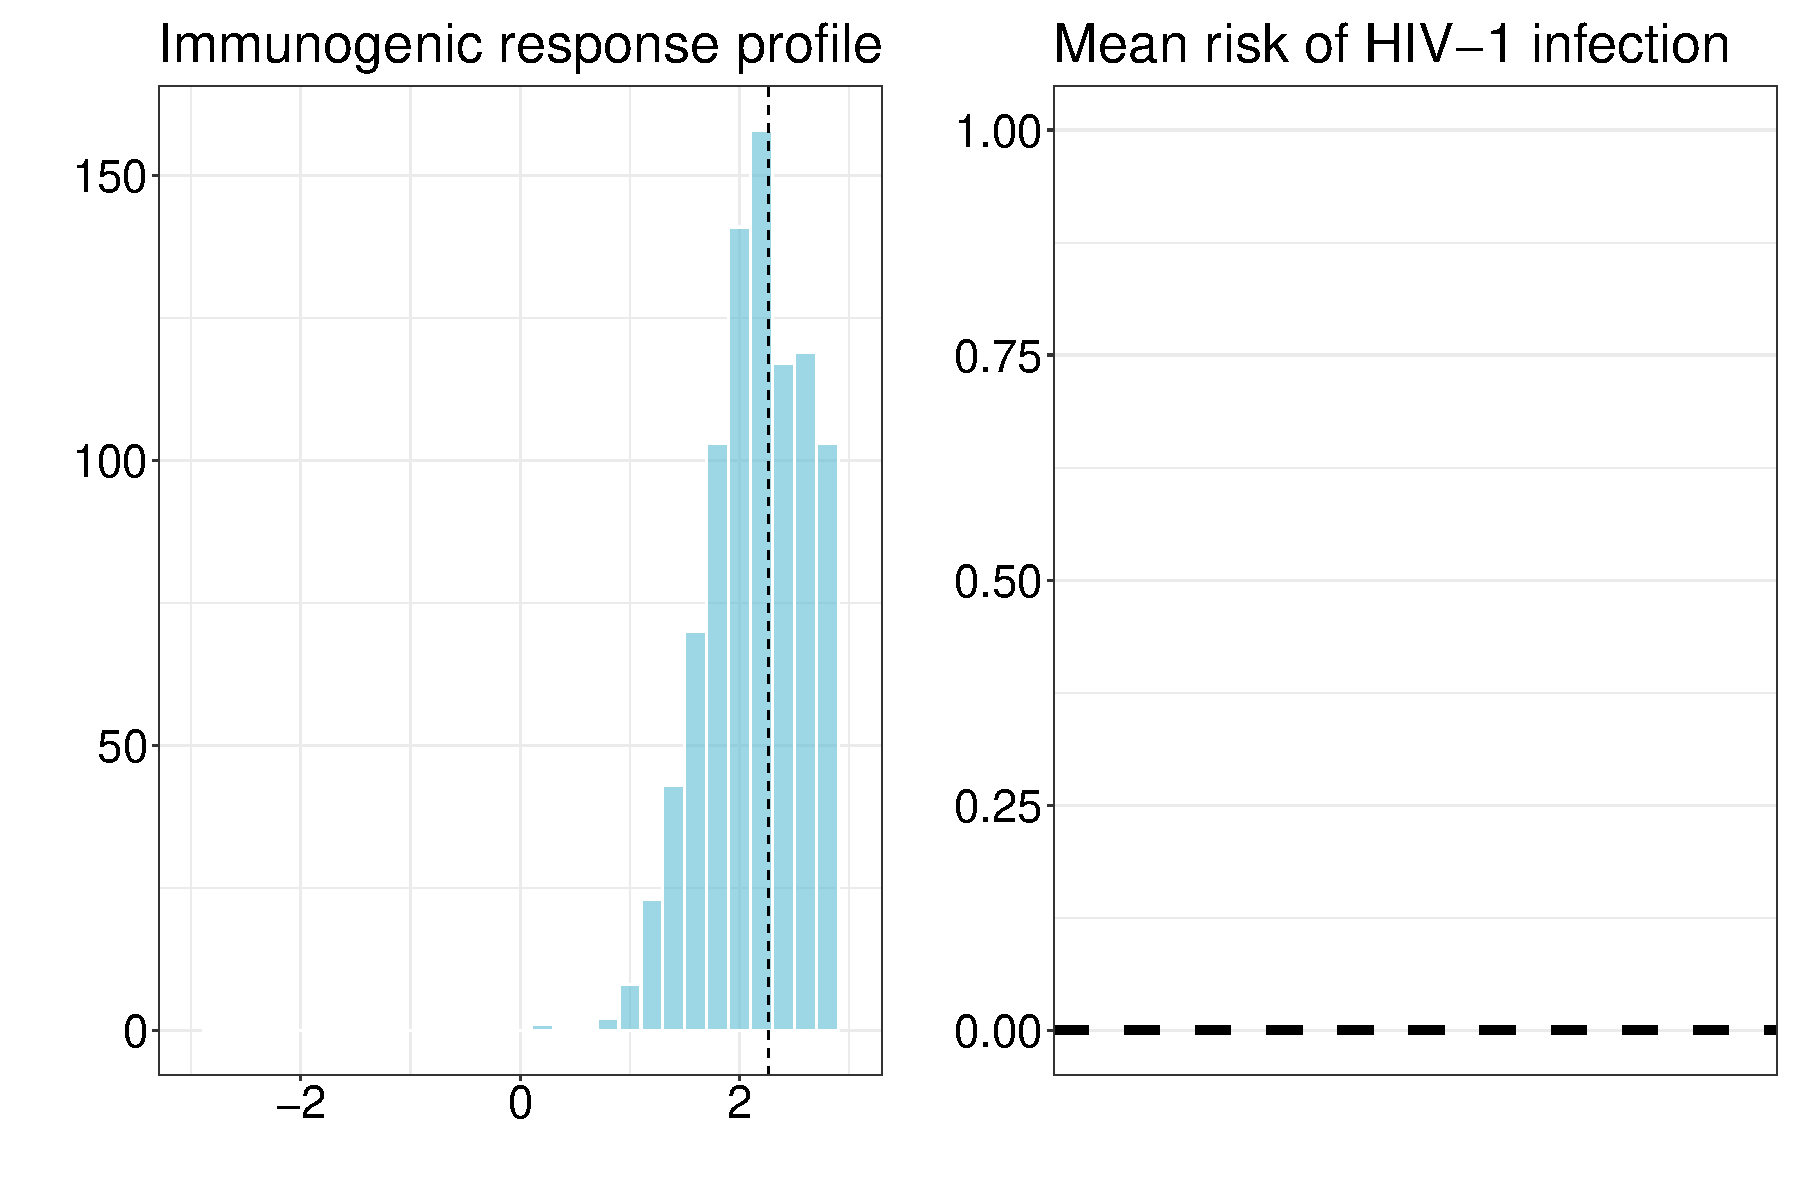
\includegraphics[scale=0.4]{shift-10}

\note{
}

\end{frame}

%%%%%%%%%%%%%%%%%%%%%%%%%%%%%%%%%%%%%%%%%%%%%%%%%%%%%%%%%%%%%%%%%%%%%%%%%%%%%%%%

\begin{frame}[c]{Flexible, efficient estimation}

\begin{center}
\begin{itemize}
  \itemsep10pt
  \item The efficient influence function (EIF) is:
    \begin{equation*}
      D(P_0^X)(x) = H(s, l)({y - \overline{Q}(s, l)}) +
      \overline{Q}(d(s, l), l) - \Psi(P_0^X).
    \end{equation*}
  \item The one-step estimator corrects bias by adding the empirical mean of the
    estimated EIF to the substitution estimator:
    \begin{equation*}\label{tmle}
        \Psi_n^{+} = \frac{1}{n} \sum_{i = 1}^n \overline{Q}_n(d(S_i, L_i),
        L_i) + D_n(O_i).
      \end{equation*}
  \item The TML estimator updates initial estimates of $\overline{Q}_n$ by
      tilting:
    \begin{equation*}\label{tmle}
      \Psi_n^{\star} = \frac{1}{n} \sum_{i = 1}^n
      \overline{Q}_n^{\star}(d(S_i, L_i), L_i).
      \end{equation*}
  \item Both estimators are doubly robust.
\end{itemize}
\end{center}

\note{
  \begin{itemize}
    \item Both estimators are CAN even when nuisance parameters are estimated
      via flexible, machine learning techniques.
    \item Semiparametric-efficient estimation thru solving efficient influence
      function estimating equation wrt the model $\M$.
    \item The auxiliary covariate simplifies when the treatment is in the limits
      (conditional on $W$) --- i.e., for $S_i \in (u(l) - \delta, u(l))$, then
      we have $H(s,l) = \frac{g_0(s - \delta \mid l)}{g_0(s \mid l)} + 1$.
    \item Need to explicitly remind the audience what $u(l)$ is again. It's only
      appeared once at this point, and only been mentioned in passing.
  \end{itemize}
}

\end{frame}

%%%%%%%%%%%%%%%%%%%%%%%%%%%%%%%%%%%%%%%%%%%%%%%%%%%%%%%%%%%%%%%%%%%%%%%%%%%%%%%%

\begin{frame}[c]{Augmented estimators for two-phase sampling designs}

\begin{center}
\begin{itemize}
  \itemsep10pt
  \item \cite{rose2011targeted2sd} introduce the IPCW-TMLE, to be used when
    observed data is subject to two-phase sampling.
  \item \textit{Initial proposal:} correct for two-phase sampling by using a
    loss function with inverse probability of censoring weights:
    \begin{equation*}
      \lik(P_0^X)(O) = \frac{C}{\pi_0(Y, L)}\lik^F(P_0^X)(X)
    \end{equation*}
  \item When the sampling mechanism $\pi_0(Y,L)$ can be estimated by
    a parametric form, this procedure yields an efficient estimator.
  \item However, when machine learning is used (e.g., when $\pi_0(Y,L)$ is not
    \textit{known by design}), this is insufficient.
\end{itemize}
\end{center}

\note{
}

\end{frame}

%%%%%%%%%%%%%%%%%%%%%%%%%%%%%%%%%%%%%%%%%%%%%%%%%%%%%%%%%%%%%%%%%%%%%%%%%%%%%%%%

\begin{frame}[c]{Efficient estimation and multiple robustness}

\begin{center}
\begin{itemize}
  \itemsep10pt
  \item Then, the IPCW augmentation must be applied to the EIF:
    \begin{align*}
      D(P_0^X)(o) = &\frac{c}{\pi_0(y, l)} D^F(P_0^X)(x) - \left(1 -
        \frac{c}{\pi_0(y, l)}\right) \cdot \\ &\E(D^F(P_0^X)(x) \mid
        C = 1, Y = y, L = l),
    \end{align*}
   \begin{itemize}
    \itemsep6pt
     \item Expresses observed data EIF $D^F(P_0^X)(o)$ in terms of full data
       EIF $D^F(P_0^X)(x)$; inclusion of second term ensures efficiency.
     \item The expectation of the full data EIF $D^F(P_0^X)(x)$, taken only over
      units selected by the sampling mechanism (i.e., $C = 1$).
  \end{itemize}
 \item A unique multiple robustness property --- combinations of
    $(g_0(L), \overline{Q}_0(S,L)) \times (\pi_0(Y, L), \E(D^F(P^X_0)(x) \mid
    C = 1, Y, L))$.
\end{itemize}
\end{center}

\note{
}

\end{frame}

%%%%%%%%%%%%%%%%%%%%%%%%%%%%%%%%%%%%%%%%%%%%%%%%%%%%%%%%%%%%%%%%%%%%%%%%%%%%%%%%

\begin{frame}[c]{Fighting the HIV-1 epidemic with preventive vaccines}

%\vspace{-1.5em}
\begin{figure}[H]
  \centering
  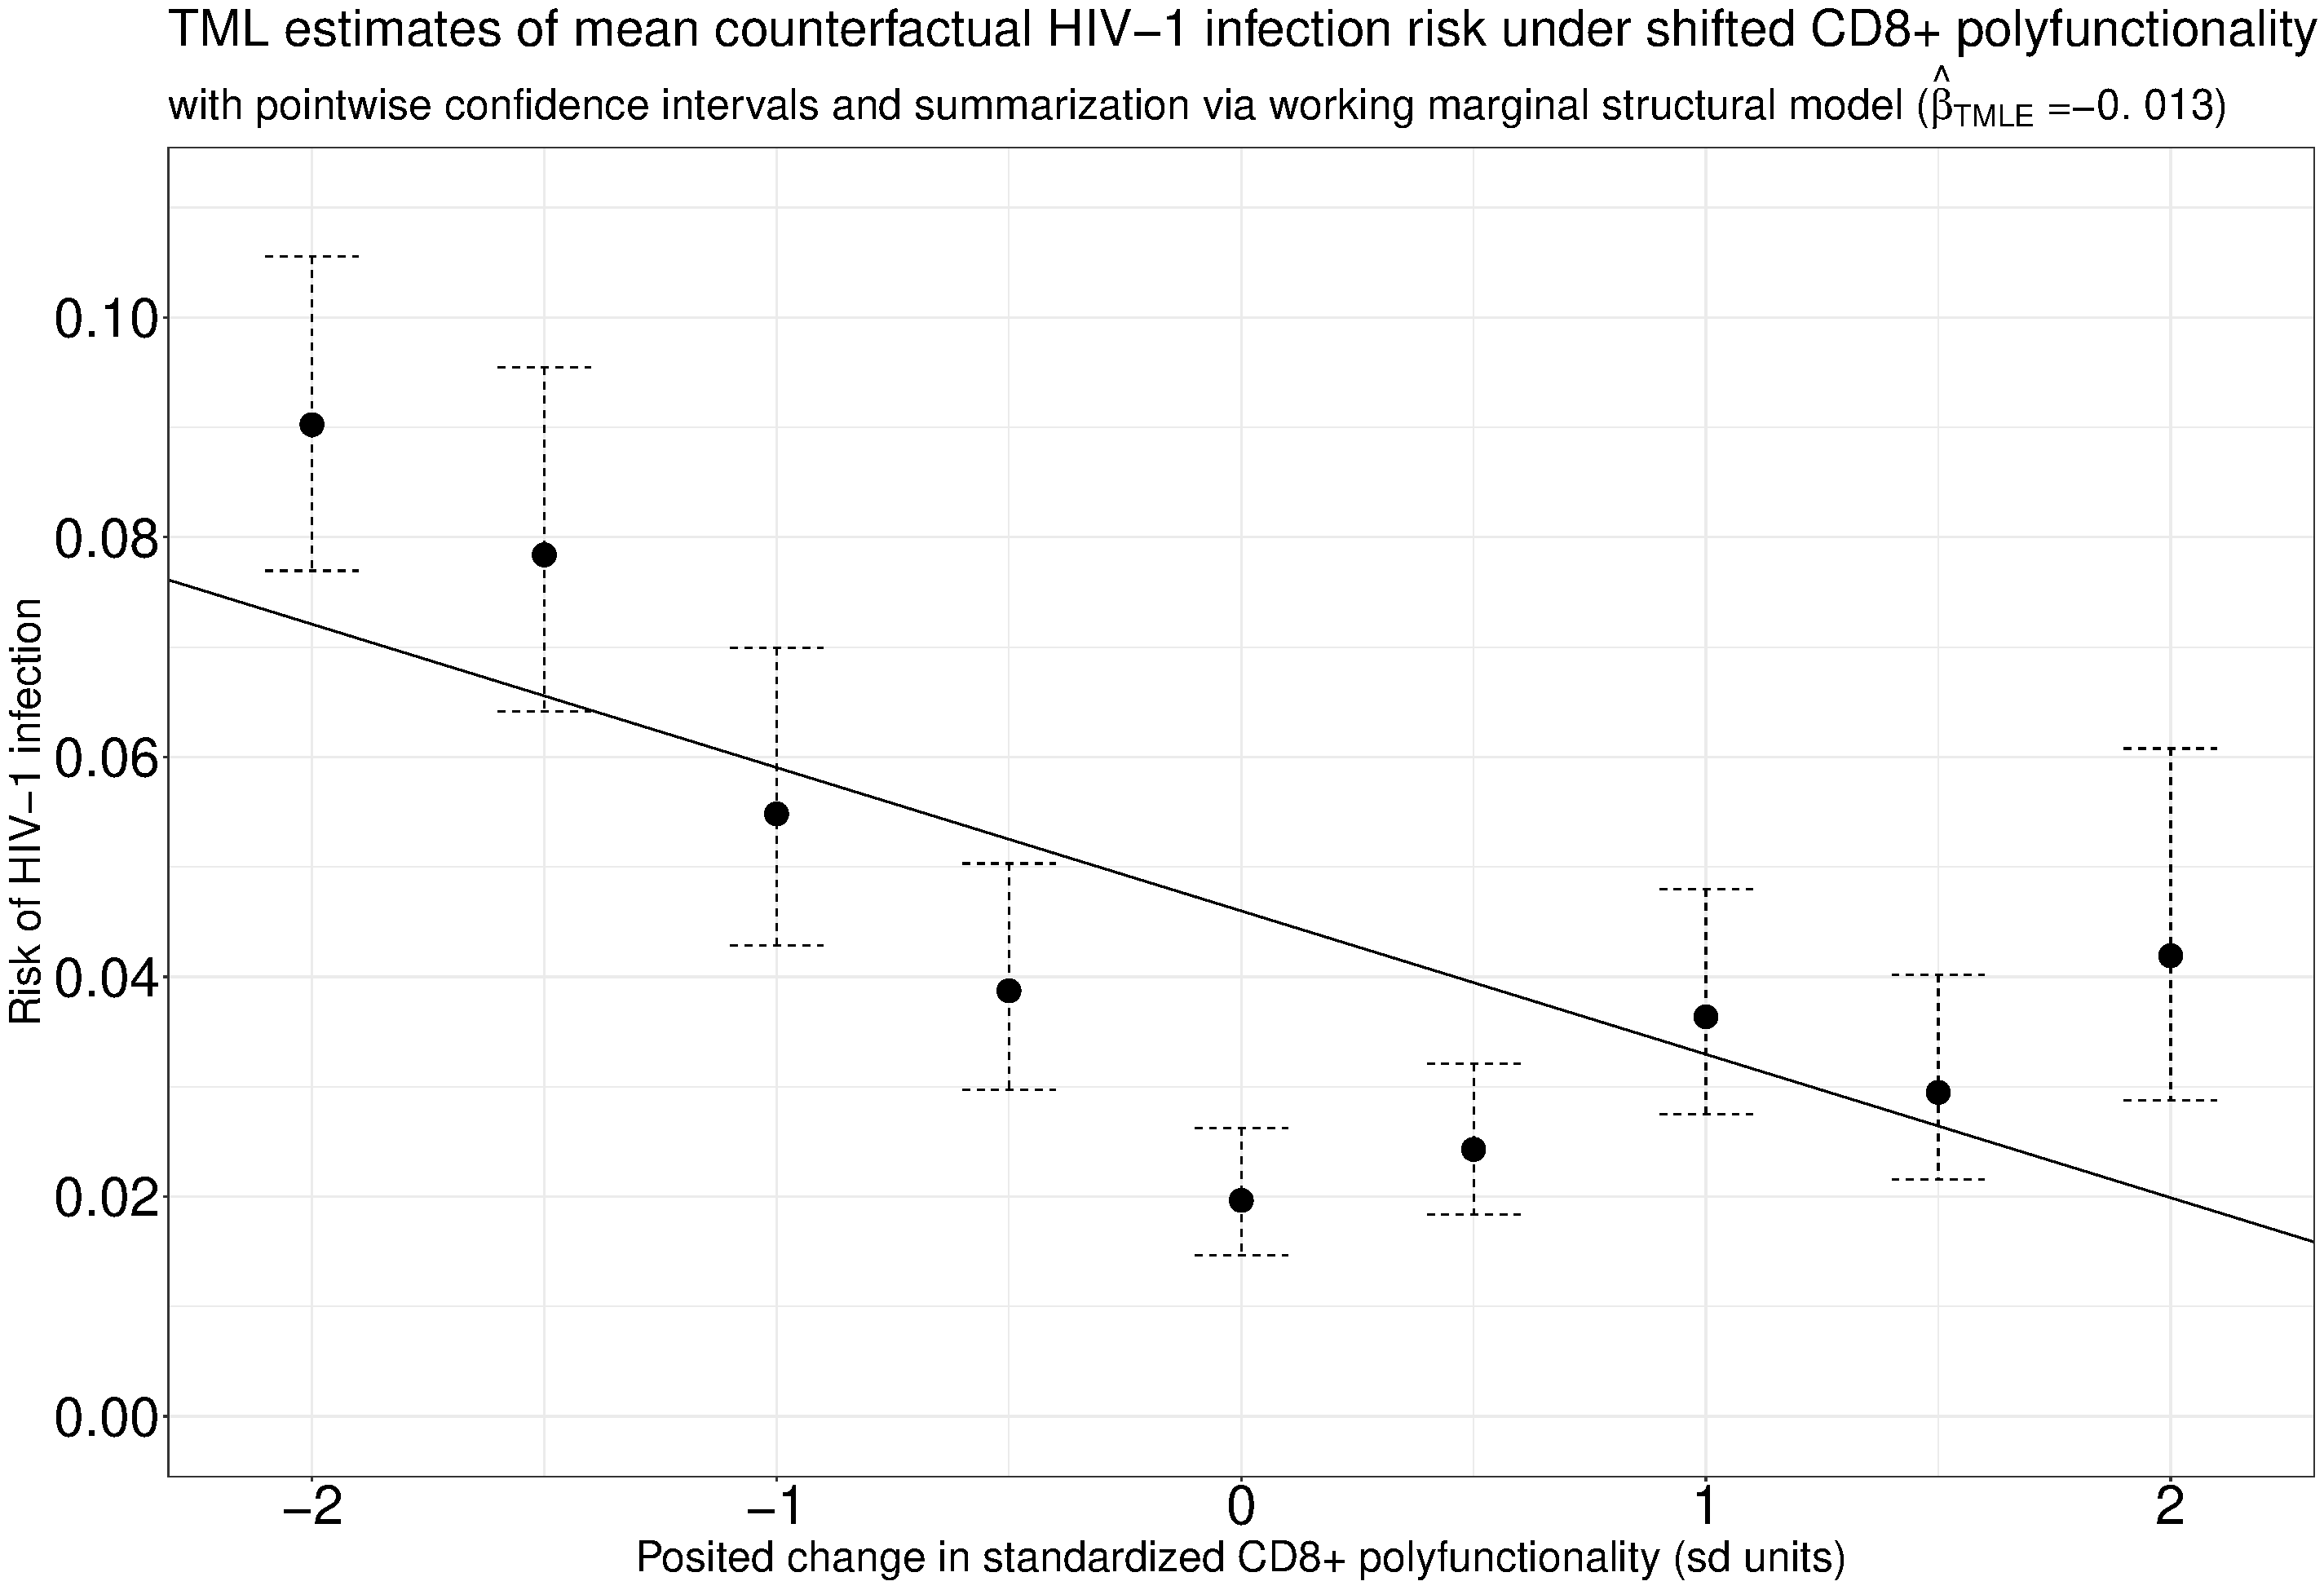
\includegraphics[scale=0.19]{cd8_msm_tmle_summary}
  \caption{
    Analysis of HIV-1 risk as a function of CD8+ immunogenicity, using
    \texttt{R} package \texttt{txshift}
    (\url{https://github.com/nhejazi/txshift}.)
  }
\end{figure}

\note{
}

\end{frame}

%%%%%%%%%%%%%%%%%%%%%%%%%%%%%%%%%%%%%%%%%%%%%%%%%%%%%%%%%%%%%%%%%%%%%%%%%%%%%%%%

\begin{frame}[c]{Big picture takeaways}

\begin{center}
\begin{itemize}
  \itemsep8pt
  \item Vaccine efficacy evaluation helps to develop enhanced vaccines better
    informed by biological properties of the target disease.
  \item HIV-1 vaccines modulate immunogenic response profiles as part of their
    mechanism for lowering HIV-1 infection risk.
  \item \textit{Stochastic} interventions constitute a flexible framework for
    considering \textbf{realistic} treatment/intervention policies.
  \item Large-scale (vaccine) trials often use two-phase designs --- need to
    (carefully!) accommodate for sampling complications.
  \item We've developed robust, open source statistical software for assessing
    stochastic interventions in observational studies.
\end{itemize}
\end{center}

\note{
}

\end{frame}

%%%%%%%%%%%%%%%%%%%%%%%%%%%%%%%%%%%%%%%%%%%%%%%%%%%%%%%%%%%%%%%%%%%%%%%%%%%%%%%%%%

\begin{frame}[c]{Thank you!}

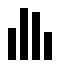
\includegraphics[scale=0.14]{homepage.png} \url{https://nimahejazi.org}

\vspace{2mm}

\includegraphics[scale=0.14]{twitter-icon.png}
  \url{https://twitter.com/nshejazi}

\vspace{2mm}
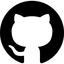
\includegraphics[scale=0.11]{github-icon.png}
  \url{https://github.com/nhejazi}

\vspace{2mm}

\includegraphics[scale=0.14]{paper-icon.png}
  \url{https://doi.org/10.1111/biom.13375}

\end{frame}

%%%%%%%%%%%%%%%%%%%%%%%%%%%%%%%%%%%%%%%%%%%%%%%%%%%%%%%%%%%%%%%%%%%%%%%%%%%%%%

\begin{frame}[standout]
  At Warp Speed -- COVID-19 Vaccine Trials
\end{frame}

%%%%%%%%%%%%%%%%%%%%%%%%%%%%%%%%%%%%%%%%%%%%%%%%%%%%%%%%%%%%%%%%%%%%%%%%%%%%%%%%

\begin{frame}[c]{COVID-19 Vaccine Development}

\begin{center}
\begin{itemize}
  \itemsep10pt
  \item \textit{Nucleic acid vaccines}: Moderna (mRNA), Pfizer (mRNA)
  \item \textit{Viral-vectored vaccines}: AstraZeneca (chimpanzee adenovirus),
     Janssen (human adenovirus)
  \item \textit{Subunit vaccines}: NovaVax, Sanofi / GlaxoSmithKline
  \item \textit{Weakened/inactivated vaccines}: Sinopharm, Sinovac
\end{itemize}
\end{center}

\note{
  \begin{itemize}
    \item Nucleic acid vaccines have never been approved before, but are quick
      to manufacture.
    \item Viral-vectored vaccines are also quick to manufacture but can develop
      immunity against vector.
  \item Subunit vaccines are a construct of several effective vaccines, but are
      slower to manufacture and often require an adjuvant.
  \end{itemize}
}

\end{frame}

%%%%%%%%%%%%%%%%%%%%%%%%%%%%%%%%%%%%%%%%%%%%%%%%%%%%%%%%%%%%%%%%%%%%%%%%%%%%%%%%

\begin{frame}[c]{Operation Warp Speed (OWS)}

\begin{center}
\begin{itemize}
  \itemsep10pt
  \item Do we have the time? Polio (7 years), Measles (9 years), Chickenpox (34
     years), Mumps (4 years), HPV (15 years).
  \item OWS: ``300M doses of safe, effective vaccine by 01 Jan.~2021''.
  \item How? Typical process timeline (73 months) replaced by an
      \textit{accelerated} process of 14 months.
  \item COVID-19 Prevention Network (CoVPN):
      \begin{itemize}
          \item formed by NIAID to establish a unified clinical trial network
              for evaluating vaccines and monoclonal antibodies.
          \item Statisticians: primary trial design/analysis,
          sequential efficacy monitoring, safety monitoring,
          \underline{immune correlates}.
      \end{itemize}
\end{itemize}
\end{center}

\note{
}

\end{frame}

%%%%%%%%%%%%%%%%%%%%%%%%%%%%%%%%%%%%%%%%%%%%%%%%%%%%%%%%%%%%%%%%%%%%%%%%%%%%%%%%

\begin{frame}[c]{Immune Correlates of
  Protection~\citep{plotkin2012nomenclature}}

\begin{center}
\begin{itemize}
  \itemsep10pt
  \item Correlate of Protection (CoP): immune marker statistically predictive
    of vaccine efficacy, not necessarily mechanistic.
  \item Mechanistic CoP (mCoP): immune marker that is causally and
    mechanistically responsible for protection.
  \item Nonmechanistic CoP (nCoP): immune marker that is predictive but not a
    causal agent of protection.
  \item A CoP is a \textit{candidate surrogate}
      endpoint~\citep{prentice1989surrogate} --- primary
      endpoint in future trials if reliably predictive.
\end{itemize}
\end{center}

\note{
}

\end{frame}

%%%%%%%%%%%%%%%%%%%%%%%%%%%%%%%%%%%%%%%%%%%%%%%%%%%%%%%%%%%%%%%%%%%%%%%%%%%%%%%%

\begin{frame}[c]{Measuring Correlates: Two-Phase Designs}

\begin{center}
\begin{itemize}
  \itemsep10pt
    \item Running assays on $>30,000$ blood draws is timely, expensive, and,
      as it turns out, statistically unnecessary.
    \item Instead we measure immune responses via a case-cohort
      design~\citep{prentice1986case}:
      \begin{itemize}
          \item a stratified random subcohort ($\approx 1600$ individuals)
          \item all SARS-CoV-2 and COVID endpoints.
      \end{itemize}
    \item Case-cohort designs are a special case of two-phase
      sampling~\citep{breslow2003large,breslow2009improved}:
      \begin{itemize}
          \item Phase 1: measure baseline, vaccine, endpoint on everyone.
          \item Phase 2: given baseline, vaccine, endpoint, select members of
            immune response subcohort with (possibly known) probability.
      \end{itemize}
\end{itemize}
\end{center}

\note{
}

\end{frame}

%%%%%%%%%%%%%%%%%%%%%%%%%%%%%%%%%%%%%%%%%%%%%%%%%%%%%%%%%%%%%%%%%%%%%%%%%%%%%%%%

\begin{frame}[c]{Stochastic--Interventional Vaccine Efficacy}

\begin{center}
\begin{itemize}
  \itemsep10pt
  \item Causal parameter based on vaccine efficacy (VE) estimands:
  \begin{equation*}
    \text{SVE}(\delta) = 1 - \frac{\E[\pr(Y = 1 \mid A = 1,
        S = s + \delta, X = x) \mid A = 1, X]}{\pr(Y(0)=1)}.
  \end{equation*}
  \item $\pr(Y(0)=1)$: counterfactual infection risk in the placebo arm ---
     under randomization, $\pr(Y(0)=1) = \pr(Y=1 \mid A=0)$.
  \item Summarizes VE thru stochastic interventions indexed by $\delta$.
  \item Further details in CoVPN's public immune correlates SAP at
      \url{https://doi.org/10.6084/m9.figshare.13198595}.
\end{itemize}
\end{center}

\note{
}

\end{frame}

%%%%%%%%%%%%%%%%%%%%%%%%%%%%%%%%%%%%%%%%%%%%%%%%%%%%%%%%%%%%%%%%%%%%%%%%%%%%%%%%

\begin{frame}[c]{Additional Complexities of Two-Phase Designs}

\begin{center}
\begin{itemize}
  \itemsep10pt
  \item Observed data structure: $O = (L, A, Z, CS, Y, C)$
      \begin{itemize}
          \item $A \in \{0, 1\}$: randomized vaccination assignment
          \item $Z$: post-vaccination confounder (e.g., unblinded risky behavior)
          \item $S$: candidate mCoPs (causal mediators)
          \item $Y$: symptomatic SARS-CoV-2 infection
          \item $C \coloneqq f(Y, L)$: selection into second-phase sample
      \end{itemize}
  \item But what about $O = (L, A, Z, CS, \Delta, \widetilde{T}, C)$?
      \begin{itemize}
          \item $\widetilde{T} = \min(T_F, T_C)$: possibly right-censored time
              to infection
          \item $\Delta = \mathbb{I}(T_F < T_C)$: symptomatic SARS-CoV-2 infection
          \item Can $C$ still be a function of $\widetilde{T}$?
      \end{itemize}
\end{itemize}
\end{center}

\note{
  \begin{itemize}
  \item Goal: assess \textit{indirect} effect of vaccination through mCoPs.
  \item Define/identify new mCoPs to be used as surrogate endpoints.
  \item Could also have missing outcome in the binary endpoint case.
  \end{itemize}
}

\end{frame}

%%%%%%%%%%%%%%%%%%%%%%%%%%%%%%%%%%%%%%%%%%%%%%%%%%%%%%%%%%%%%%%%%%%%%%%%%%%%%%%%

\begin{frame}[c]{Causal Mediation Analysis: Explanation and Mechanism}

\begin{center}
\begin{itemize}
  \itemsep 10pt
  \item Identification assumptions:
      \begin{itemize}
          \item A1: No unmeasured confounding of $\{A, Y\}$ relationship.
          \item A2: No unmeasured confounding of $\{S, Y\}$ relationship.
          \item A3: No unmeasured confounding of $\{A, S\}$ relationship.
        \item A4: No $\{S, Y\}$ confounder affected by $A$, i.e., no $Z$.
      \end{itemize}
  \item \textit{Indirect} effects: thru pathways involving candidate mCoPs.
      \begin{itemize}
          \item Natural (in)direct effects~\citep{robins1992identifiability,
              pearl2013direct}: binary $A$ and $S$, no $Z$, ``cross-world''
              independence.
          \item Stochastic (in)direct effects~\citep{diaz2020causal}:
          continuous $A$ and $S$, no $Z$; no ``cross-world'' exclusion.
          \item Interventional (in)direct effects~\citep{diaz2020nonparametric}:
          binary $A$, continuous $S$, $Z$ OK, no ``cross-world'' exclusion.
          \item Stochastic interventional (in)direct
            effects~\citep{hejazi2020nonparametric}:
          continuous $A$ and $S$, $Z$ ok, no ``cross-world'' exclusion.
      \end{itemize}

\end{itemize}
\end{center}

\note{
  \begin{itemize}
  \item A1, A3 hold in randomized trials.
  \item A2 may not hold: include all mutual $\{S, Y\}$ predictors, then perform
      sensitivity analysis.
  \item A4 usually doesn't hold: either measure $S$ right after $A$ or develop
      more flexible effect definitions.
  \item ``Cross-world'' independence: $Y(a, s) \perp S(a') \quad \forall s$;
     untestable in RCTs
  \item Extensions for two-phase sampling?
  \end{itemize}
}

\end{frame}

%%%%%%%%%%%%%%%%%%%%%%%%%%%%%%%%%%%%%%%%%%%%%%%%%%%%%%%%%%%%%%%%%%%%%%%%%%%%%%%%

\appendix
\begin{frame}[standout]
  Appendix
\end{frame}

%%%%%%%%%%%%%%%%%%%%%%%%%%%%%%%%%%%%%%%%%%%%%%%%%%%%%%%%%%%%%%%%%%%%%%%%%%%%%%%%

\begin{frame}[c]{Literature: \cite{haneuse2013estimation}}

\begin{center}
\begin{itemize}
  \itemsep10pt
  \item \textit{Proposal:} Characterization of stochastic interventions as
    \textit{modified treatment policies} (MTPs).
  \item Assumption of \textit{piecewise smooth invertibility} allows for the
    intervention distribution of any MTP to be recovered:
    \begin{equation*}
      g_{0, \delta}(s \mid l) = \sum_{j = 1}^{J(l)} I_{\delta, j} \{h_j(s, l),
      l\} g_0\{h_j(s, l) \mid l\} h^{'}_j(s,l)
    \end{equation*}
  \item Such intervention policies account for the natural value of the
    intervention $S$ directly yet are interpretable as the imposition of an
    altered intervention mechanism.
  \item Identification conditions for assessing the parameter of interest under
    such interventions appear technically complex (at first).
\end{itemize}
\end{center}

\note{
  \begin{itemize}
    \item Shifts of the form $d(S,L)$ are considerably more interesting since
      these are realistic intervention policies.
    \item Example: consider an individual with an extremely high immune response
      but whose baseline covariates $L$ suggest we shift the response still
      higher. Such a shift may not be biologically plausible (impossible, even)
      but we cannot account for this if the shift is only a function of $L$.
    \item The authors build IPW, outcome regression, and non-iterative doubly
      robust estimators, as well as an approach based on MSMs.
    \item Piecewise smooth invertibility: This assumption ensures that we can
      use the change of variable formula when computing integrals over $S$ and
      it is useful to study the estimators that we propose in this paper.
  \end{itemize}
}

\end{frame}

%%%%%%%%%%%%%%%%%%%%%%%%%%%%%%%%%%%%%%%%%%%%%%%%%%%%%%%%%%%%%%%%%%%%%%%%%%%%%%%%

\begin{frame}[c]{Literature: \cite{young2014identification}}

\begin{center}
\begin{itemize}
  \itemsep10pt
  \item Establishes equivalence between g-formula when proposed intervention
    depends on natural value and when it does not.
  \item This equivalence leads to a sufficient positivity condition for
    estimating the counterfactual mean under MTPs via the same statistical
    functional studied in \cite{diaz2012population}.
  \item Extends earlier identification results, providing a way to use the same
    statistical functional to assess $\E Y_{d(S,L)}$ or $\E Y_{d(L)}$.
  \item The authors also consider limits on implementing shifts $d(S,L)$, and
    address working in a longitudinal setting.
\end{itemize}
\end{center}

\note{
}

\end{frame}

%%%%%%%%%%%%%%%%%%%%%%%%%%%%%%%%%%%%%%%%%%%%%%%%%%%%%%%%%%%%%%%%%%%%%%%%%%%%%%%%

\begin{frame}[c]{Literature: \cite{diaz2018stochastic}}

\begin{center}
\begin{itemize}
  \itemsep10pt
  \item Builds on the original proposal, accomodating MTP-type shifts $d(S,L)$
    proposed after their earlier work.
  \item To protect against positivity violations, considers a specific shifting
    mechanism:
     \begin{equation*}\label{shift_intervention}
       d(s, l) =
         \begin{cases}
           s + \delta, & s + \delta < u(l) \\
           s, & \text{otherwise}
         \end{cases}
     \end{equation*}
  \item Proposes an improved TMLE algorithm, with a single auxiliary
    covariate for constructing the TML estimator.
\end{itemize}
\end{center}

\note{
}

\end{frame}

%%%%%%%%%%%%%%%%%%%%%%%%%%%%%%%%%%%%%%%%%%%%%%%%%%%%%%%%%%%%%%%%%%%%%%%%%%%%%%%%

\begin{frame}[c]{Nonparametric conditional density estimation}

\begin{center}
\begin{itemize}
  \itemsep8pt
  \item To compute the auxiliary covariate $H(s,l)$, we need to estimate
    conditional densities $g(S \mid L)$ and $g(S - \delta \mid L)$.
  \item There is a rich literature on density estimation, we follow the approach
    proposed in \cite{diaz2011super}.
  \item To build a conditional density estimator, consider
    \begin{equation*}
      g_{n, \alpha}(s \mid L) = \frac{\pr (S \in [\alpha_{t-1}, \alpha_t)
        \mid L)}{\alpha_t - \alpha_{t-1}},
    \end{equation*}
    for $\alpha_{t-1} \leq s < \alpha_t$.
    \vspace{0.5em}
    \begin{itemize}
      \itemsep4pt
      \item This is a classification problem, where we estimate the probability
        that a value of $S$ falls in a bin $[\alpha_{t-1}, \alpha_t)$.
      \item The choice of the tuning parameter $t$ corresponds roughly to the
        choice of bandwidth in classical kernel density estimation.
    \end{itemize}
\end{itemize}
\end{center}

\note{
}

\end{frame}

%%%%%%%%%%%%%%%%%%%%%%%%%%%%%%%%%%%%%%%%%%%%%%%%%%%%%%%%%%%%%%%%%%%%%%%%%%%%%%%%

\begin{frame}[c]{Nonparametric conditional density estimation}

\begin{center}
\begin{itemize}
  \itemsep8pt
  \item \cite{diaz2011super} propose a reformulation of this classification
    approach as a set of hazard regressions.
  \item To effectively employ this proposed reformulation, consider
    \begin{align*}
      \pr(S \in [\alpha_{t-1}, \alpha_t) \mid L) =& \pr (S \in [\alpha_{t-1},
      \alpha_t) \mid S \geq \alpha_{t-1}, L) \times  \\ & \Pi_{j = 1}^{t-1}
      \{1 - \pr(S \in [\alpha_{j-1}, \alpha_j) \mid S \geq \alpha_{j-1}, L) \}
    \end{align*}
    \vspace{0.25em}
    \begin{itemize}
      \itemsep4pt
      \item The likelihood of this model may be expressed to correspond to the
        likelihood of a binary variable in a data set expressed via a long-form
        repeated measures structure.
      \item Specifically, the observation of $X_i$ is repeated as many times as
        intervals $[\alpha_{t-1}, \alpha_t)$ are before the interval to which
        $S_i$ belongs, and the binary variables indicating $S_i \in
        [\alpha_{t-1}, \alpha_t)$ are recorded.
    \end{itemize}
\end{itemize}
\end{center}

\note{
}

\end{frame}

%%%%%%%%%%%%%%%%%%%%%%%%%%%%%%%%%%%%%%%%%%%%%%%%%%%%%%%%%%%%%%%%%%%%%%%%%%%%%%%%

\begin{frame}[c]{Density estimation with the Super Learner algorithm}

\begin{center}
\begin{itemize}
  \itemsep10pt
  \item To estimate $g(S \mid L$) and $g(S - \delta \mid L)$, use a pooled
    hazard regression, spanning the support of $S$.
  \item We rely on the Super Learner algorithm of \cite{vdl2007super} to build
    an ensemble learner that optimally weights each of the proposed regressions,
    using cross-validation (CV).
  \item The Super Learner algorithm uses $V$-fold CV to train each proposed
    regression model, weighting each by the inverse of its average risk across
    all $V$ holdout sets.
  \item By using a library of regression estimators, we invoke the result of
    \cite{vdl2004asymptotic}, who prove this likelihood-based cross-validated
    estimator to be asymptotically optimal.
\end{itemize}
\end{center}

\note{
\begin{itemize}
  \item The auxiliary covariate simplifies when the treatment is in the limits
    (conditional on $L$) --- i.e., for $S_i \in (u(l) - \delta, u(l))$, then we
    have $H(s,l) = \frac{g_0(s - \delta \mid l)}{g_0(s \mid l)} + 1$.
  \item Asymptotically optimal in the sense that it performs as well as the
    oracle selector as the sample size increases.
\end{itemize}
}

\end{frame}

%%%%%%%%%%%%%%%%%%%%%%%%%%%%%%%%%%%%%%%%%%%%%%%%%%%%%%%%%%%%%%%%%%%%%%%%%%%%%%%%

\begin{frame}[c]{Key properties of TML estimators}

\begin{center}
\begin{itemize}
  \itemsep10pt
  \item \textbf{Asymptotic linearity:}
    \begin{equation*}
      \Psi(P_n^{\star}) - \Psi(P_0^X) = \frac{1}{n} \sum_{i = 1}^{n}
      D(P_0^X)(X_i) + o_P\left(\frac{1}{\sqrt{n}}\right)
    \end{equation*}
  \item \textbf{Gaussian limiting distribution:}
    \begin{equation*}
      \sqrt{n}(\Psi(P_n^{\star}) - \Psi(P_0^X)) \to N(0, Var(D(P_0^X)(X)))
    \end{equation*}
  \item \textbf{Statistical inference:}
    \begin{equation*}
      \text{Wald-type confidence interval}: \Psi(P_n^{\star}) \pm z_{1 -
      \frac{\alpha}{2}} \cdot \frac{\sigma_n}{\sqrt{n}},
    \end{equation*}
    where $\sigma_n^2$ is computed directly via
    $\sigma_n^2 = \frac{1}{n} \sum_{i = 1}^{n} D^2(\cdot)(X_i)$.
\end{itemize}
\end{center}

\note{
Under the additional condition that the remainder term $R(\hat{P}^{\star},
P_0)$ decays as $o_P \left( \frac{1}{\sqrt{n}} \right),$ we have that
$\Psi_n - \Psi_0 = (P_n - P_0) \cdot D(P_0) + o_P
\left( \frac{1}{\sqrt{n}} \right),$ which, by a central limit theorem,
establishes a Gaussian limiting distribution for the estimator, with variance
$V(D(P_0))$, the variance of the efficient influence function
when $\Psi$ admits an asymptotically linear representation.

The above implies that $\Psi_n$ is a $\sqrt{n}$-consistent estimator of $\Psi$,
that it is asymptotically normal (as given above), and that it is locally
efficient. This allows us to build Wald-type confidence intervals, where
$\sigma_n^2$ is an estimator of $V(D(P_0))$. The estimator $\sigma_n^2$
may be obtained using the bootstrap or computed directly via
$\sigma_n^2 = \frac{1}{n} \sum_{i = 1}^{n} D^2(\bar{Q}_n^{\star}, g_n)(O_i)$

We obtain semiparametric-efficient estimation and robust inference in the
nonparametric model $\M$ by solving the efficient influence function.

\begin{enumerate}
   \item If $D(\bar{Q}_n^{\star}, g_n)$ converges to $D(P_0)$ in $L_2(P_0)$ norm.
   \item The size of the class of functions $\bar{Q}_n^{\star}$ and $g_n$ is
     bounded (technically, $\exists \mathcal{F}$
     s.t.~$D(\bar{Q}_n^{\star}, g_n) \in \mathcal{F}$ w.h.p., where
     $\mathcal{F}$ is a Donsker class)
\end{enumerate}
}

\end{frame}

%%%%%%%%%%%%%%%%%%%%%%%%%%%%%%%%%%%%%%%%%%%%%%%%%%%%%%%%%%%%%%%%%%%%%%%%%%%%%%%%

\begin{frame}[c]{Algorithm for TML estimation}

\begin{center}
\begin{enumerate}\label{tmle_algo}
  \itemsep6pt
  \item Construct initial estimators $g_n$ of $g_0(S, L)$ and $Q_n$ of
    $\overline{Q}_0(S, L)$, perhaps using data-adaptive regression techniques.
  \item For each observation $i$, compute an estimate $H_n(s_i, l_i)$ of the
    auxiliary covariate $H(s_i, l_i)$.
  \item Estimate the parameter $\epsilon$ in the logistic regression model
    $$\text{logit}\overline{Q}_{\epsilon, n}(s, l) =
    \text{logit}\overline{Q}_n(s, l) + \epsilon H_n(s, l),$$
    or an alternative regression model incorporating weights.
  \item Compute TML estimator $\Psi_n$ of the target parameter, defining update
    $\overline{Q}_n^{\star}$ of the initial estimate
    $\overline{Q}_{n, \epsilon_n}$:
    \begin{equation*}\label{tmle}
      \Psi_n = \Psi(P_n^{\star}) = \frac{1}{n} \sum_{i = 1}^n
        \overline{Q}_n^{\star}(d(S_i, L_i), L_i).
      \end{equation*}
\end{enumerate}
\end{center}

\note{
  \begin{itemize}
    \item We recommend using nonparametric methods for the initial estimators,
      as consistent estimation is necessary for efficiency of the estimator
      $\Psi_n$.
    \item Intuition for the submodel fluctuation?
  \end{itemize}
}

\end{frame}

%%%%%%%%%%%%%%%%%%%%%%%%%%%%%%%%%%%%%%%%%%%%%%%%%%%%%%%%%%%%%%%%%%%%%%%%%%%%%%%%

\begin{frame}[c]{Algorithm for IPCW-TML estimation}

\begin{center}
\begin{enumerate}\label{ipcwtmle_algo}
  \itemsep8pt
  \item Using all observed units ($X$), estimate sampling mechanism
    $\pi(Y, L)$, perhaps using data-adaptive regression methods.
  \item Using only observed units in the second-stage sample $C = 1$,
    construct initial estimators $g_n(S,L)$ and $\overline{Q}_n(S,L)$,
    weighting by the sampling mechanism estimate $\pi_n(Y,L)$.
  \item With the approach described for the full data case, compute
    $H_n(s_i,l_i)$, and fluctuate submodel via logistic regression.
  \item Compute IPCW-TML estimator $\Psi_n$ of the target parameter, by solving
    the IPCW-augmented EIF estimating equation.
  \item Iteratively update estimated sampling weights $\pi_n(Y,L)$ and
    IPCW-augmented EIF, updating TML estimate in each iteration, until
    $\frac{1}{n}\sum_{i = 1}^n \text{EIF}_i < \frac{1}{n}$.
\end{enumerate}
\end{center}

\note{
  \begin{itemize}
    \item We recommend using nonparametric methods for the initial estimators,
      as consistent estimation is necessary for efficiency of the estimator
      $\Psi_n$.
    \item Intuition for the submodel fluctuation?
    \item This process includes the use of HAL to fit the regression of the EIF
      contributions on the sampling node $\{Y, L\}$.
  \end{itemize}
}

\end{frame}

%%%%%%%%%%%%%%%%%%%%%%%%%%%%%%%%%%%%%%%%%%%%%%%%%%%%%%%%%%%%%%%%%%%%%%%%%%%%%%%%

\begin{frame}[c]{Identifying the best efficient estimator}

%\vspace{-1.5em}
\begin{figure}[H]
  \centering
  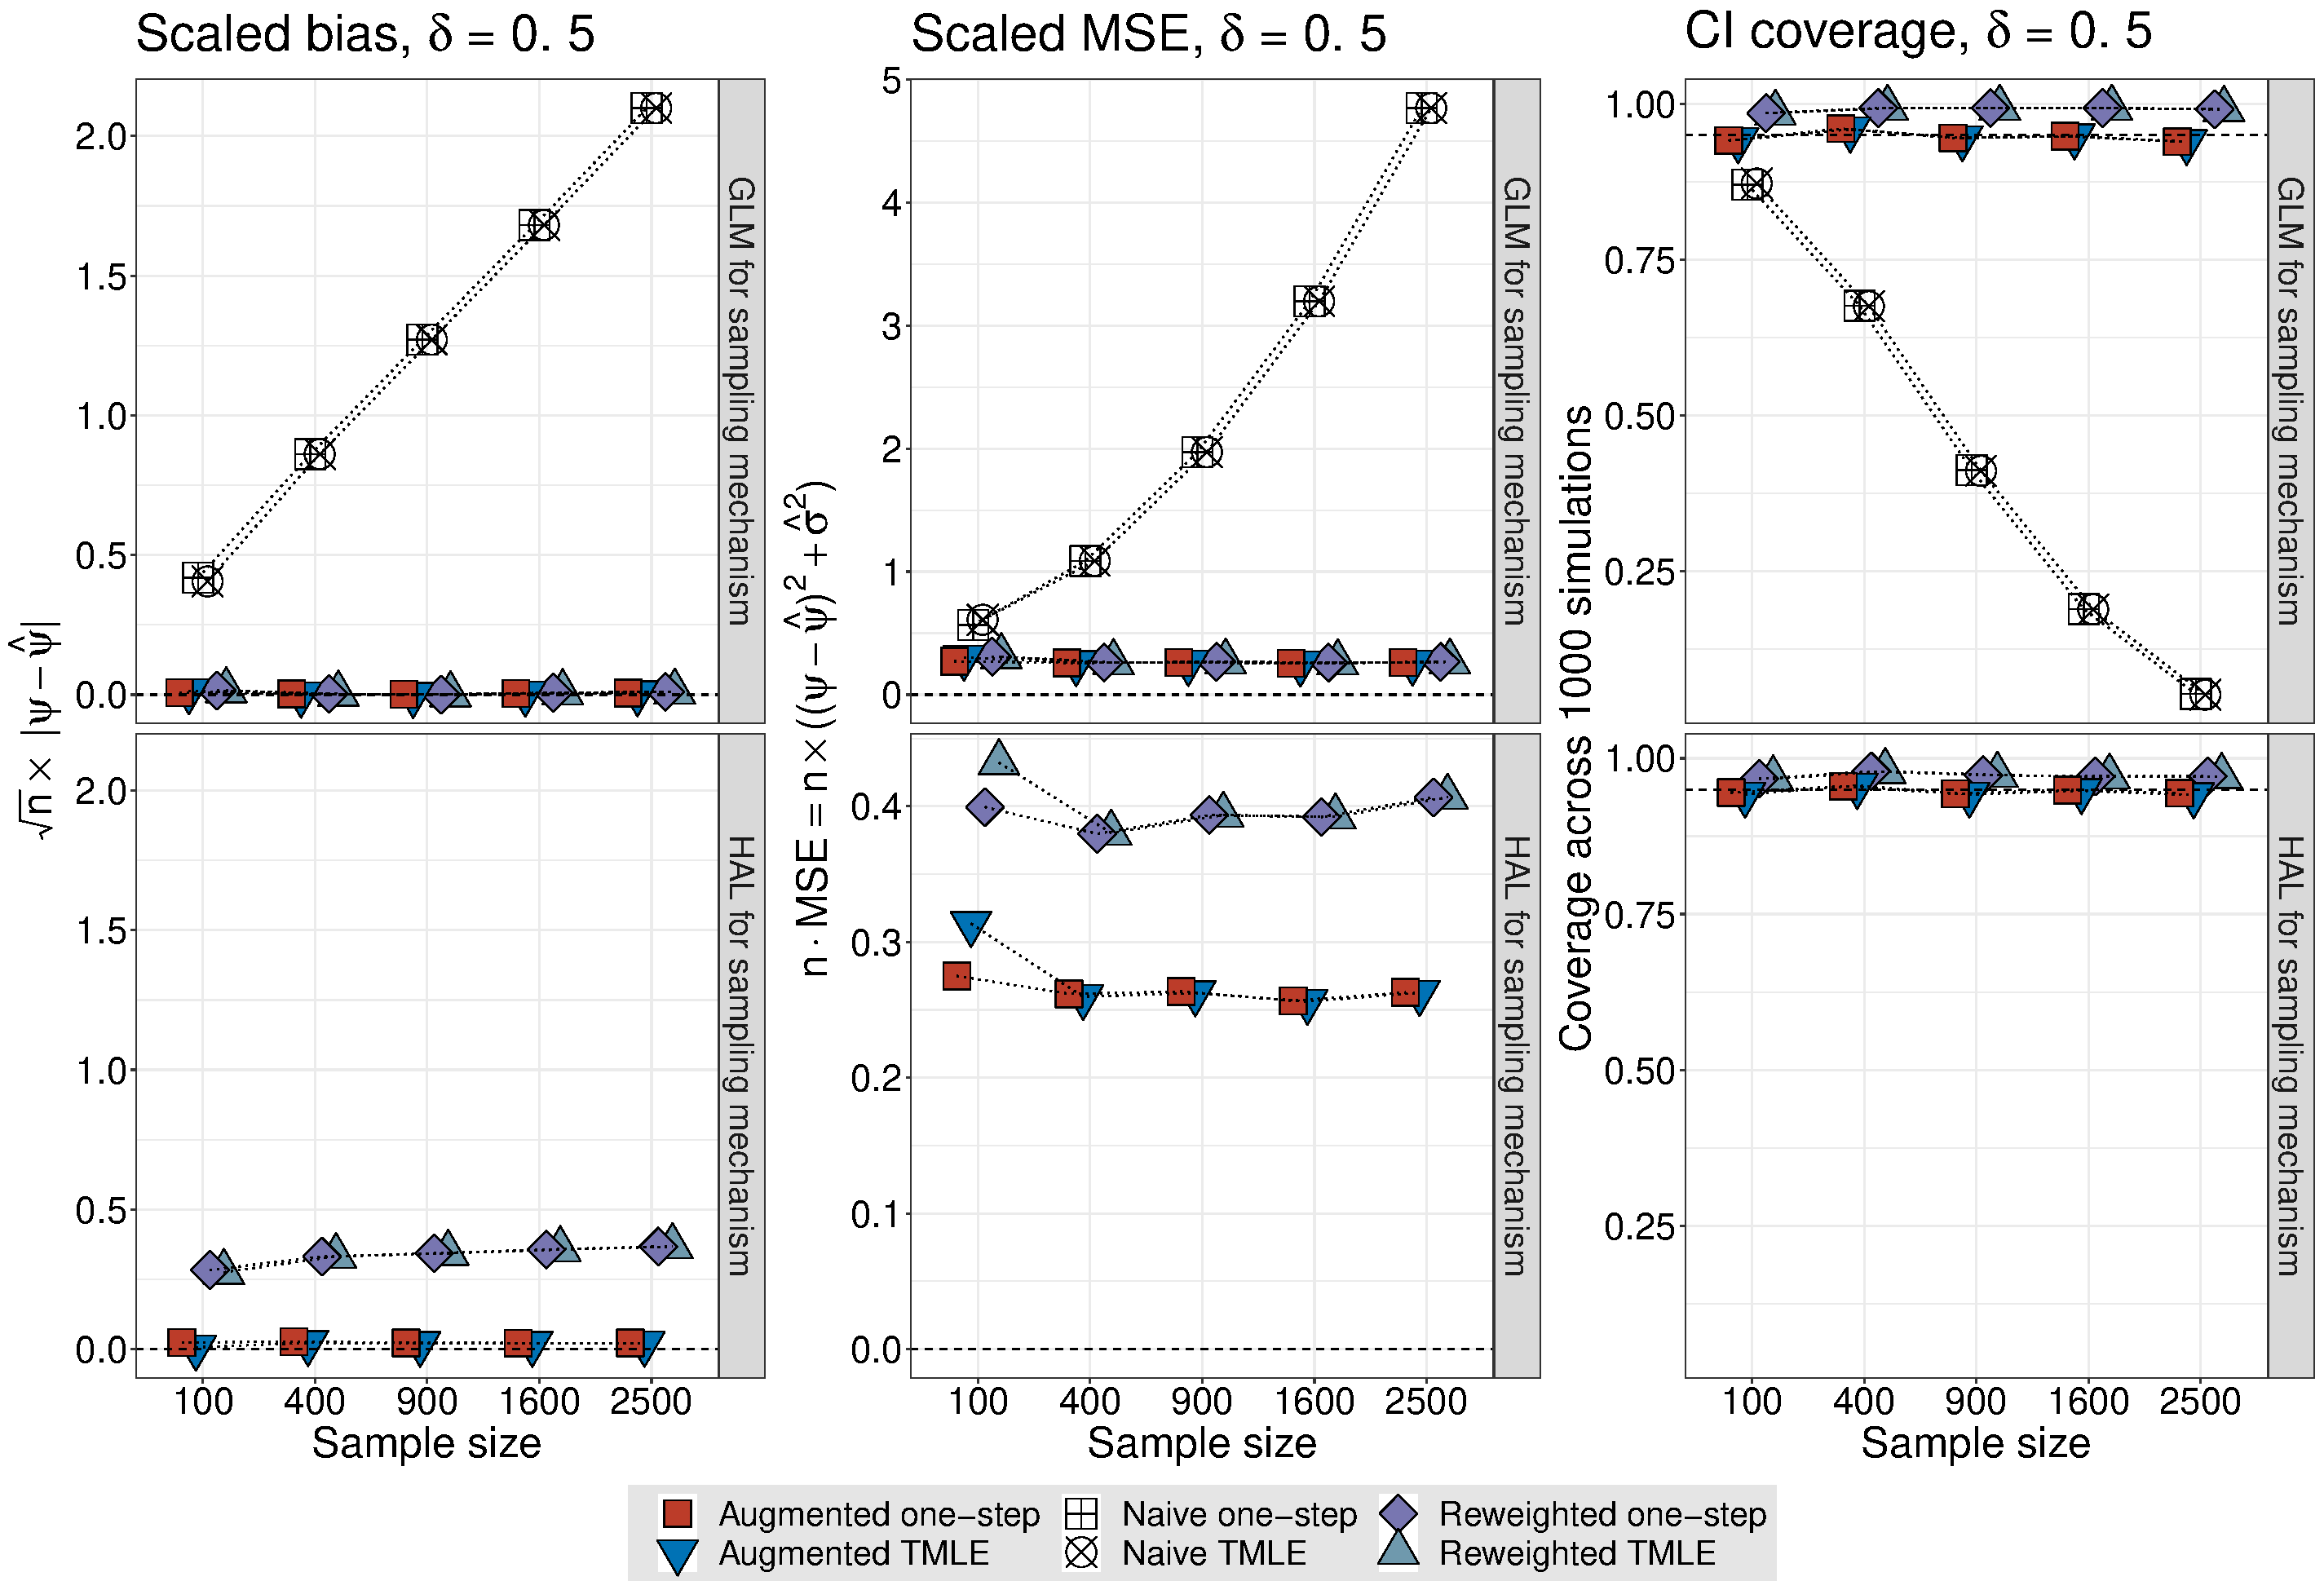
\includegraphics[scale=0.22]{simple_effect_panel_delta_upshift}
  \caption{
    Relative performance of reweighted and augmented estimators.
  }
\end{figure}

\note{
}

\end{frame}

%%%%%%%%%%%%%%%%%%%%%%%%%%%%%%%%%%%%%%%%%%%%%%%%%%%%%%%%%%%%%%%%%%%%%%%%%%%%%%%%

\begin{frame}[c]{A linear modeling perspective}

\begin{center}
\begin{itemize}
  \itemsep6pt
  \item Briefly consider a simple data structure: $X = (Y, S)$; we seek to model
    the outcome $Y$ as a function of $S$.
  \item To posit a linear model, consider $Y_i = \beta_0 + \beta_1 S_i +
    \epsilon_i$, with error $\epsilon_i \sim N(0, 1)$.
  \item Letting $\delta$ be a change in $S$, $Y_{S + \delta} - Y_S$ may be
    expressed
    \begin{align*}
      \E Y_{S + \delta} - \E Y_S &= [\beta_0 + \beta_1 (\E S + \delta)] -
        [\beta_0 + \beta_1 (\E S)] \\
        &= \beta_0 - \beta_0 + \beta_1 \E S - \beta_1 \E S + \beta_1 \delta \\
        &= \beta_1 \delta
    \end{align*}
  \item Thus, a \textit{unit shift} in $S$ (i.e., $\delta = 1$) may be seen as
    inducing a change in the difference in outcomes of magnitude $\beta_1$.
\end{itemize}
\end{center}

\note{
  \begin{itemize}
    \item We extend this result to the mean counterfactual outcomes under the
      nonparametric model $\M$.
  \end{itemize}
}

\end{frame}

%%%%%%%%%%%%%%%%%%%%%%%%%%%%%%%%%%%%%%%%%%%%%%%%%%%%%%%%%%%%%%%%%%%%%%%%%%%%%%%%

\begin{frame}[c]{A causal inference perspective}

\begin{center}
\begin{itemize}
  \itemsep6pt
  \item Consider a data structure: $(Y_s, s \in \mathcal{S})$.
  \item To posit a linear model, let $Y_s = \beta_0 + \beta_1 s
    + \epsilon_s$ for $s \in \mathcal{S}$, with error
    $\epsilon_s \sim N(0, \sigma^2_s)$ $\forall s \in S$.
  \item For the counterfactual outcomes $(Y_{s' + \delta}, Y_{s'})$, their
    difference, $Y_{s' + \delta} - Y_{s'}$, for some $s' \in \mathcal{S}$, may
    be expressed
    \begin{align*}
      \E Y_{s' + \delta} - \E Y_{s'} &= [\beta_0 + \beta_1 (s' + \delta) +
          \E \epsilon_{s' + \delta}] - [\beta_0 + \beta_1 s' +
          \E \epsilon_{s'}] \\
        &= \beta_1 \delta
    \end{align*}
  \item Thus, a \textit{unit shift} for $s' \in S$ (i.e., $\delta = 1$) may be
    seen as inducing a change in the difference in the counterfactual outcomes
    of magnitude $\beta_1$.
\end{itemize}
\end{center}

\note{
  \begin{itemize}
    \item Note that this analysis is exactly what we're told we \textbf{cannot}
      do in ``linear models 101'' --- that is, the slope of a regression line cannot
      be interpreted as \textit{causing} a change in the outcome.
    \item We extend this result to the mean counterfactual outcomes under the
      nonparametric model $\M$.
  \end{itemize}
}

\end{frame}

%%%%%%%%%%%%%%%%%%%%%%%%%%%%%%%%%%%%%%%%%%%%%%%%%%%%%%%%%%%%%%%%%%%%%%%%%%%%%%%%

\begin{frame}[c]{Slope in a semiparametric model}

\begin{center}
\begin{itemize}
  \itemsep10pt
  \item Consider the stochastic intervention $g^{\star}(\cdot \mid L)$:
    \begin{align*}
      \E Y_{g^{\star}} &= \int_L \int_s \E(Y \mid S = s, L) g(s - \delta
            \mid L) \cdot ds \cdot dP_0(L) \\
        &= \int_L \int_z \E(Y \mid S = z + \delta, L) g(z \mid L) \cdot dz
          \cdot dP_0(L),
    \end{align*}
      defning the change of variable $z = s - \delta$.
  \item For a semiparametric model, $\E (Y \mid S = z, L) = \beta z +
    \theta(L)$:
    \begin{align*}
      \E Y_{g^{\star}} - \E Y &= \int_L \int_z
      \begin{aligned}[t]
        & [\E(Y \mid S = z + \delta, L) - \E(Y \mid S = z, L)] \\
        & g(z \mid L) \cdot dz \cdot dP_0(L)
      \end{aligned} \\
      &= [\beta (z + \delta) + \theta(L)] - [\beta z + \theta(L)] \\
      &= \beta \delta
    \end{align*}
\end{itemize}
\end{center}

\note{
}

\end{frame}

%%%%%%%%%%%%%%%%%%%%%%%%%%%%%%%%%%%%%%%%%%%%%%%%%%%%%%%%%%%%%%%%%%%%%%%%%%%%%%%%

% don't want dimming with references
\setbeamercovered{}
\beamerdefaultoverlayspecification{}

\begin{frame}[c,allowframebreaks]{}

\small
\bibliographystyle{apalike}
\nocite{*}
\bibliography{references}
%\itemize

\end{frame}

%%%%%%%%%%%%%%%%%%%%%%%%%%%%%%%%%%%%%%%%%%%%%%%%%%%%%%%%%%%%%%%%%%%%%%%%%%%%%%%%

\end{document}
